% Format teze zasnovan je na paketu memoir
% http://tug.ctan.org/macros/latex/contrib/memoir/memman.pdf ili
% http://texdoc.net/texmf-dist/doc/latex/memoir/memman.pdf
% 
% Prilikom zadavanja klase memoir, navedenim opcijama se podešava 
% veličina slova (12pt) i jednostrano štampanje (oneside).
% Ove parametre možete menjati samo ako pravite nezvanične verzije
% mastera za privatnu upotrebu (na primer, u b5 varijanti ima smisla 
% smanjiti 
\documentclass[12pt,oneside]{memoir}

% Paket koji definiše sve specifičnosti mastera Matematičkog fakulteta
\usepackage{matfmaster}
%
% Podrazumevano pismo je ćirilica.
%   Ako koristite pdflatex, a ne xetex, sav latinički tekst na srpskom jeziku
%   treba biti okružen sa \lat{...} ili \begin{latinica}...\end{latinica}.
%
% Opicija [latinica]:
%   ako želite da pišete latiniciom, dodajte opciju "latinica" tj.
%   prethodni paket uključite pomoću: \usepackage[latinica]{matfmaster}.
%   Ako koristite pdflatex, a ne xetex, sav ćirilički tekst treba biti
%   okružen sa \cir{...} ili \begin{cirilica}...\end{cirilica}.
%
% Opcija [biblatex]:
%   ako želite da koristite reference na više jezika i umesto paketa
%   bibtex da koristite BibLaTeX/Biber, dodajte opciju "biblatex" tj.
%   prethodni paket uključite pomoću: \usepackage[biblatex]{matfmaster}
%
% Opcija [b5paper]:
%   ako želite da napravite verziju teze u manjem (b5) formatu, navedite
%   opciju "b5paper", tj. prethodni paket uključite pomoću: 
%   \usepackage[b5paper]{matfmaster}. Tada ima smisla razmisliti o promeni
%   veličine slova (izmenom opcije 12pt na 11pt u \documentclass{memoir}).
%
% Naravno, opcije je moguće kombinovati.
% Npr. \usepackage[b5paper,biblatex]{matfmaster}

% Pomoćni paket koji generiše nasumičan tekst u kojem se javljaju sva slova
% azbuke (nema potrebe koristiti ovo u pravim disertacijama)
\usepackage{pangrami}

% Paket koji obezbeđuje ispravni prikaz ćiriličkih italik slova kada
% se koristi pdflatex. Zakomentarisati ako na sistemu koji koristite ovaj
% paket nije dostupan ili ako ne radi ispravno.
\usepackage{cmsrb}

% Ostali paketi koji se koriste u dokumentu
\usepackage{listings} % listing programskog koda

\renewcommand\lstlistingname{К\^{о}д}
\renewcommand\lstlistlistingname{К\^{о}д}

\usepackage{xcolor}

\definecolor{codegreen}{rgb}{0,0.6,0}
\definecolor{codegray}{rgb}{0.5,0.5,0.5}
\definecolor{codepurple}{rgb}{0.58,0,0.82}
\definecolor{backcolour}{rgb}{0.94,0.94,0.94}

\lstdefinestyle{mystyle}{
    basicstyle=\sffamily,
    backgroundcolor=\color{backcolour},   
    commentstyle=\color{codegreen},
    keywordstyle=\color{red},
    numberstyle=\tiny\color{codegray},
    stringstyle=\color{codepurple},
    breakatwhitespace=false,         
    breaklines=true,                 
    captionpos=b,                    
    keepspaces=true,                 
    %numbers=left,                    
    numbersep=5pt,                  
    showspaces=false,                
    showstringspaces=false,
    showtabs=false,                  
    tabsize=2
}

\lstset{style=mystyle}

% Datoteka sa literaturom u BibTex tj. BibLaTeX/Biber formatu
\bib{matfmaster-primer}

% Ime kandidata na srpskom jeziku (u odabranom pismu)
\autor{Давид Гавриловић}
% Naslov teze na srpskom jeziku (u odabranom pismu)
\naslov{Дистрибуирана обрада геопросторних података}
% Godina u kojoj je teza predana komisiji
\godina{2022}
% Ime i afilijacija mentora (u odabranom pismu)
\mentor{др Милена Вујошевић Јаничић, ванредни професор\\ Универзитет у Београду, Математички факултет}
% Ime i afilijacija prvog člana komisije (u odabranom pismu)
\komisijaA{др Саша Малков, ванредни професор\\ Универзитет у Београду, Математички факултет}
% Ime i afilijacija drugog člana komisije (u odabranom pismu)
\komisijaB{др Mирко Спасић, доцент\\ Универзитет у Београду, Математички факултет}
% Ime i afilijacija trećeg člana komisije (opciono)
% \komisijaC{}
% Ime i afilijacija četvrtog člana komisije (opciono)
% \komisijaD{}
% Datum odbrane (obrisati ili iskomentarisati narednu liniju ako datum odbrane nije poznat)
\datumodbrane{10. јун 2022.}

% Apstrakt na srpskom jeziku (u odabranom pismu)
\apstr{%
\pangrami
}

% Ključne reči na srpskom jeziku (u odabranom pismu)
\kljucnereci{анализа, геометрија, алгебра, логика, рачунарство, астрономија}

\begin{document}
% ==============================================================================
% Uvodni deo teze
\frontmatter
% ==============================================================================
% Naslovna strana
\naslovna
% Strana sa podacima o mentoru i članovima komisije
\komisija
% Strana sa posvetom (u odabranom pismu)
\posveta{некоме}
% Strana sa podacima o disertaciji na srpskom jeziku
\apstrakt
% Sadržaj teze
\tableofcontents*

% ==============================================================================
% Glavni deo teze
\mainmatter
% ==============================================================================


\chapter{Увод}
\label{chp:uvod}

увод о свему у раду

\textbf{TODO}

\chapter{Програмски језик Скала}
\label{chp:scala}

Скала (енг. Scala) је виши програмски језик заснован на функционалној и објектно оријентисаној парадигми. Име је добила од енглеске речи \textit{scalable} јер је дизајнирана тако да се развија са потребама корисника. Има широк спектар примена и може се користити за писање једноставних скрипти али и у изградњи великих и комплексних система. \cite{scala_prog}

Настала је 2001. на швајцарском федералном институту за технологију у Лозани (фра. \textit{École Polytechnique Fédérale de Lausanne}) и њен творац је Мартин Одерски (енг. \textit{Martin Odersky}). Прва званична верзија је изашла 20. јануара 2004. године.

Данас је широко распрострањена и користе је велике корпорације, као што су \textit{Twitter}, \textit{Google} и \textit{Apple}. Поред тога, веома је заступљена у заједници отвореног кода у пројектима као што су \textit{Apache Spark}, \textit{Apache Kafka}, \textit{Apache Flink} и \textit{Akka}.

\section{Особине језика \textit{Scala}}
\label{sec:osоб_scala}

\textit{Scala} је спој две парадигме, објектно оријентисане и функционалне, па стога поседује велики број особина. Поред тога, компајлира се на исти начин као и језик Јава, са којим постоје одређене сличности.

\subsection{Објектно оријентисан и функционалан језик}
\label{subsec:scala_obj_prog}

Скала је у потпуности објектно оријентисан језик. То значи да је свака вредност која се дефинише објекат, као и да је свака акција која се позива метод. На пример, уколико се врши одузимање два цела броја, позива се метод назван $''-''$ (минус). Тај метод је дефинисан у класи која представља целе бројеве, \textit{Int}. \cite{scala_prog}

Поред тога што је објектно оријентисан језик, \textit{Scala} је и функционалан језик. Функционално програмирање је засновано на два принципа. Први је да су функције вредности првог реда. То значи да се функције посматрају на исти начин као и други типови, на пример целобројни или ниска. Такође, функције је могуће прослеђивати другим функцијама, функције могу бити повратна вредност неке друге функције и функције се могу складиштити у променљивама.

Други принцип је да функције које се позивају немају бочне ефекте. Једна функција има улогу само да пресликава улаз у одговарајући излаз. То значи да ће сваки позив једне функције са истом вредношћу улазних аргумената, увек резултовати истом излазном вредношћу, независно од тога када се функција позива током извршавања програма. Другачији назив за ову особину је транспарентост референци. \cite{scala_prog}

Из овога произилази да функционални језици користе имутабилне структуре података. То су такве структуре за које важи да се подаци унутар њих не мењају. Уколико до промене мора доћи, сама структура се не мења, већ се од ње конструише тотално нова, са измењеним вредностима. \cite{scala_prog}

Међутим, Скала није чисто функционалан језик, што значи да се ипак може дефинисати функција која поседује бочне ефекте или се могу користити структуре података које се могу мењати. Поред тога, Скала омогућава писање функционалног кода без бочних ефеката и са имутабилним структурама података, па се може користити и на тај начин. \cite{scala_prog}

\subsection{Повезаност са језиком Јава}
\label{subsec:scala_komp}

\textit{Scala} је конструисана тако да се компајлира у Јавин ЈВМ бајтк\^{о}д (енг. \textit{Java JVM bytecode}). То значи да \textit{Scala} може користити Јава класе, методе и типове. На пример, Скалин објектни целобројни тип у својој имплементацији користи примитивни еквивалент из Јаве. Поред тога, Скала може користити Јава к\^{о}д и обогатити га на неки начин, као на пример додавањем неке методе у већ постојећу класу. Напоменимо и то да је време извршавања Скала програма приближно извршавању Јава програмима. \cite{scala_prog}

Међутим, иако се компајлирају на исти начин, програми написани у језику Скала често садрже мањи број линија од оних написаних у језику Јава. У неким случајевима се очекује да је к\^{о}д чак дупло краћи. Краћи програми доводе до тога да је к\^{о}д лакше писати и разумети, али и до мање вероватноће прављења грешака. \cite{scala_prog}

Један од многих примера како Скала смањује број линија у односу на Јаву је приказан у кодовима \ref{lst:scala_java_class_declaration} и \ref{lst:scala_scala_class_declaration} који представљају начине декларисања класе у та два програмска језика.

\begin{lstlisting}[caption={Декларација класе у језику Јава}, language=Java, label={lst:scala_java_class_declaration}]
// Java
class MyClass {  
  private int index;
  private String name;
  
  public MyClass(int index, String name) {
    this.index = index;
    this.name = name;
  }
}
\end{lstlisting}

\begin{lstlisting}[caption={Декларација класе у језику Scala}, language=Scala, label={lst:scala_scala_class_declaration}]
// Scala
class MyClass(index: Int, name: String)

\end{lstlisting}

У Скали се не мора декларисати посебна конструктор фукција, што доводи до смањења броја линија кода. \cite{scala_prog}

\subsection{Статичка типизираност}
\label{subsec:scala_stat_tip}

Статичка типизираност значи да се типови променљивих закључују за време компилације програма. То је супротно од динамичке типизираности која то чини за време извршавања. Оба приступа имају своје предности и мане. Скала је статички типизиран језик и поседује веома напредан систем типова.

То доноси предности које доводе до лакшег откривања грешака приликом писања кода. На пример, у статички типизираним програмима се током компилације сазнаје да ли је примењена нека операција на тип над којим та операција није дозвољена. Поред тога, статичка типизираност чини рефакторисање кода поузданијим. На пример, након измене метода се са сигурношћу може рећи да се повратни тип није променио. \cite{scala_prog}

Скала није само статички типизиран језик већ је и језик који аутоматски закључује типове у току компилације. На пример, када се декларише нека променљива целобројног типа, нема потребе назначити и њен тип, пошто га компајлер може аутоматски одредити. То значи да се следеће две линије кода (пример \ref{lst:scala_scala_type_declaration}) понашају еквивалентно. Исто важи и за било који други Скала тип, не само за целобројни.

\begin{lstlisting}[caption={Декларација типова}, language=Scala, label={lst:scala_scala_type_declaration}]
// primer 1
val x: Int = 10

// primer 2
val x = 10
\end{lstlisting}

Скала програмер не мора експлицитно да наводи типове, али је то  често пожељно због тога што се на тај начин осигурава да ће к\^{о}д заправо користити тип који му је намењен, али ће и побољшати читљивост и допринети документацији. \cite{scala_prog}

\section{Скала интерпретер}
\label{sec:scala_interpr}

Скала је језик који се може интерпретирати. Да би се покренуо Скала интерпретер потребно је покренути команду \textit{scala}.

\begin{lstlisting}[language=Scala, caption={Скала интерпретер}, label={lst:scala_scala_interpreter_example}]
$ scala
Welcome to Scala 2.13.6
Type in expressions for evaluation. Or try :help.

scala>
\end{lstlisting}

Након што се унесе к\^{о}д у интерпретер и притисне ентер, покреће се извршавање написаног кода и излаз се приказује у конзоли.

\begin{lstlisting}[language=Scala, caption={Пример кода у интерпретеру}, label={lst:scala_interpreter_code_example}]
scala> 20 + 100
val res0: Int = 120
\end{lstlisting}

Излаз покренуте команде је аутоматски генерисана променљива названа \textbf{res0} типа \textit{Int} у којој ће се налазити резултат унетог израчунавања. Новонастала променљива се може користити у наставку извршавања. \cite{scala_prog}

\begin{lstlisting}[language=Scala, caption={Коришћење резултатских променљивих}, label={lst:scala_res0_example}]
scala> res0 + 100
val res1: Int = 220
\end{lstlisting}

Уколико је потребно само исписати вредност у конзоли без креирања нове променљиве може се користити функција \textit{print()}.

\begin{lstlisting}[language=Scala, caption={Функција print}, label={lst:scala_interpret_print_func}]
scala> print(20 + 100)
120

scala> print("Hello!")
Hello!
\end{lstlisting}

\section{Типови}
\label{sec:scala_tip}

Сви примитивни типови Јаве имају свој одговарајући еквивалент у Скали и када се типови у Скали компајлирају у Јавин бајтк\^{о}д, превешће се баш у те типове. На пример, логички тип у Скали, \textit{scala.Boolean} је еквивалент Јавином примитивном типу \textit{boolean}. Исто важи и за друге примитивне типове Јаве попут \textit{Int}, \textit{Float} и \textit{Double}. \cite{scala_prog}

Поред њих постоје и уграђени сложени типови попут ниске (\textit{String}), н-торке (\textit{Tuple}), низа (\textit{Array}) и других. Како је Скала објектно оријентисан језик, могу се дефинисати и додатни типови уколико за тим има потребе, али о томе више речи у секцији \ref{subsec:scala_klase}.

Сваки тип, долази са скупом оператора који се на тај тип могу применити. Скала је написана тако да је сваки оператор заправо један метод дефинисан у класи која представља тип. Постоје различите врсте оператора попут аритметичких, логичких и битовских.

\section{Променљиве}
\label{sec:scala_prom}

Постоје две врсте променљивих које се дефинишу кључним речима \textit{var} и \textit{val}. Разликују се по томе што се вредност променљивих дефинисаних са \textit{val} не може мењати, док је код оних дефинисаних са \textit{var} то могуће, све док је нова додељена вредност компатибилног типа. \cite{scala_prog}

У наставку (примери \ref{lst:scala_val_reassignment}, \ref{lst:scala_var_values} и \ref{lst:scala_type_missmach}) су приказани примери дeфиниција променљивих у Скала интерпретеру.

\begin{lstlisting}[language=Scala, caption={Додељивање нове вредности val променљивима}, label={lst:scala_val_reassignment}]
scala> val x = 10
val x: Int = 10

scala> x = 20
         ^
       error: reassignment to val
\end{lstlisting}

\begin{lstlisting}[language=Scala, caption={Додељивање нове вредности var променљивима}, label={lst:scala_var_values}]
scala> var x = 10
var x: Int = 10

scala> x = 20
// mutated x

scala> x
val res0: Int = 20

\end{lstlisting}

\begin{lstlisting}[language=Scala, caption={Додељивање некомпатибилног типа}, label={lst:scala_type_missmach}]
scala> var x = 10
var x: Int = 10

scala> x = "some string"
           ^
       error: type mismatch;
        found   : String("some string")
        required: Int
\end{lstlisting}

\section{Контрола тока}
\label{sec:scala_kontr_toka}

Скала поседује уграђене стандардне наредбе за контролу тока, \textit{if} за гранање, \textit{while} за петље и \textit{for} и \textit{foreach} за итерирање кроз колекције. У наставку су те наредбе приказане у скалиној синтакси. \cite{scala_prog}

\begin{lstlisting}[language=Scala, caption={Контрола тока}, label={lst:scala_flow_control}]

if (bool izraz) {
  // izraz je evalueiran true
} else {
  // izraz je evaluiran false
}

while (bool izraz) {
  // dok se izraz ne evaluira false
}

for (element <- kolekcija) {
  // operacije nad elementom
}

kolekcija.forach(funkcija koje se poziva za svaki element kolekcije)

\end{lstlisting}

\section{Функције}
\label{sec:scala_funk}

Скала делом припада функционалној парадигми па су стога функције веома битан део језика. Функција се дефинише кључном речи \textit{def} након које редом следе име функције, опциона листа њених аргумената са њиховим типовима раздвојених зарезом, тип повратне вредности функције, знак $=$ и на крају тело функције. Пример дефиниције је приказан у коду \ref{lst:scala_function_template}.

\begin{lstlisting}[language=Scala, caption={Дефиниција фунције у скали}, label={lst:scala_function_template}]
def imeFunkcije(argument1: tip1, ...): povratni_tip = {
  // telo funkcije
}

\end{lstlisting}

У наставку је приказана функција која сабира два целобројна броја и враћа добијени резултат. 

\begin{lstlisting}[language=Scala, caption={Пример функције}, label={lst:scala_function_add_example}]
def saberi(x: Int, y: Int): Int = {
  x + y
}
\end{lstlisting}

Последња линија тела функције ће увек бити њена повратна вредност али се поред тога она може назначити и наредбом \textit{return}. Уколико се функција састоји од само једне линије кода, могу се изоставити витичасте заграде које означавају почетак и крај тела фунције. Поред тога, због закључивања типова се може изоставити и тип повратне вредности. Дакле, функција \textit{saberi()} из претходног примера се краће може записати на следећи начин:

\begin{lstlisting}[language=Scala, caption={Краћи запис функције saberi()}, label={lst:scala_function_add_example_simplified}]
scala> def saberi(x: Int, y: Int) = x + y
def saberi(x: Int, y: Int): Int

scala> saberi(40, 2)
val res0: Int = 42
\end{lstlisting}

Тип повратне вредности се у неким случајевима ипак не сме изоставити. На пример, када се користи рекурзија. Такође, функција не мора да враћа никакву вредност. У том случају је повратни тип означен са \textit{Unit}. \cite{scala_prog}

Све функције су вредности првог реда у Скали па имају и свој тип. Тип функције је представљен заградама у којима се налазе типови њених аргумената након којих следи знак $=>$ праћен типом повратне вредности. Тип функције \textit{saberi()} која поседује два аргумента типа \textit{Int}, као и исти повратни тип ће бити:

\begin{lstlisting}[language=Scala, caption={Тип функције saberi()}, label={lst:scala_function_add_example_type}]
(Int, Int) => Int
\end{lstlisting}

Експлицитно навођење типова дозвољава декларацију функција вишег реда, функција које као аргументе имају друге функције. Пример \ref{lst:scala_function_high_order_example} приказује функцију која као аргумент има функцију која има два аргумента и повратну вредност типа \textit{Int}

\begin{lstlisting}[language=Scala, caption={Функција вишег реда}, label={lst:scala_function_high_order_example}]
scala> def visiRed(f: (Int, Int) => Int, x: Int, y: Int) = {
  f(x, y)
}
def visiRed(f: (Int, Int) => Int, x: Int, y: Int): Int
\end{lstlisting}

Тип овог аргумента одговара типу функције \textit{saberi()}, па се она може проследити ново написаној функцији.

\begin{lstlisting}[language=Scala, caption={Прослеђивање функције функцији}, label={lst:scala_function_add_high_order}]
scala> visiRed(saberi, 100, 200)
val res0: Int = 300
\end{lstlisting}

Све функције које су до сада приказане су поседовале идентификатор, односно име. Међутим, то није неопходно и могуће је дефинисати функцију без имена. Такве функције се називају ламбда функције (енг. \textit{Lambda functions}).

Оне се обично користе када је нека функција потребна само једном, на пример у неком изразу, и не позива се никад више у коду. Декларишу се тако што се у заградама наводи низ аргумената са типовима, знак $=>$ и након тога повратна вредност. Пример ламбда функције која сабира два броја је приказан у наставку.

\begin{lstlisting}[language=Scala, caption={Пример ламбда функције}, label={lst:scala_function_lambda_example}]
scala> (x: Int, y: Int) => x + y
val res0: (Int, Int) => Int = $Lambda$2582/1961424035@2207eb9f
\end{lstlisting}

Ламбда функције се могу проследити функцијама вишег реда, па претходно дефинисана функција \textit{visiRed()} може бити позвана на следећи начин:

\begin{lstlisting}[language=Scala, caption={Прослеђивање ламбда функције другој функцији}, label={lst:scala_functions_lambda_high_order}]
scala> visiRed((x: Int, y: Int) => x + y, 100, 200)
val res0: Int = 300
\end{lstlisting}

У овом примеру, функција \textit{saberi()} је замењена ламбда функцијом истог понашања, што није довело до промене коначног резултата. 

\section{Објектнo оријентисана парадигма}
\label{sec:scala_oop}

У овој секцији ће детаљније бити описана објектно оријентисана парадигма језика Скала. 

\subsection{Класе}
\label{subsec:scala_klase}

Као и у Јави, у Скали класа представља нацрт преко ког се производе објекти. Да би се од класе креирао објекат, користи се кључна реч \textit{new}.

\begin{lstlisting}[language=Scala, caption={Дефиниција и инстанцирање класе у Скали}, label={lst:scala_oop_class_instance}]
scala> class MyClass {
     |     
     | }

scala> val mc = new MyClass
val mc: MyClass = MyClass@e700eba
\end{lstlisting}

Унутар класе се дефинишу поља (енг. \textit{fields}) и методе (енг. \textit{methods}), који се заједно једним именом називају чланови (енг. \textit{members}). Поља су променљиве које се дефинишу са \textit{val} или \textit{var} док су методи функције које описују неко понашање и дефинишу се на исти начин као и обичне функције. \cite{scala_prog}

\begin{lstlisting}[language=Scala, caption={Чланови класе}, label={lst:scala_oop_members_class}]
scala> class MyClass {
     |  val field = 0
     |  
     |  def method() = print(field)
     | }

scala> val mc = new MyClass
val mc: MyClass = MyClass@e700eba

scala> mc.field
mval res0: Int = 0

scala> mc.method()
0
\end{lstlisting}

Сваком члану се додељује једно правило приступа којим се одређује опсег из ког се том члану може приступити. У Скали постоје три правила приступа и то су:

\begin{description}
\item[\textit{private},] приступ унутар класе;
\item[\textit{protected},] приступ унутар класе и класа које наслеђују ту класу;
\item[\textit{public},] приступ изван класе (подразумевана вредност која се не наводи).
\end{description}

Пример \textit{private} приступа је приказан у коду \ref{lst:scala_oop_private_access}. Сваки покушај приступа приватној променљивој ван класе ће резултовати грешком.

\begin{lstlisting}[language=Scala, caption={Пример private правила приступа}, label={lst:scala_oop_private_access}]
scala> class MyClass {
     |  private val field = 0
     |    
     |  def method() = print(field)
     |  }
class MyClass

scala> val mc = new MyClass
val mc: MyClass = MyClass@6a6e9289

scala> mc.field
          ^
       error: value field in class MyClass cannot be accessed as a member of MyClass from class 
\end{lstlisting}

Поља се могу дефинисати ван тела класе, што је и Скалин стандард (к\^ od \ref{lst:scala_oop_field_outside}). Због тога се класа може написати уз помоћ мањег броја линија. 

\begin{lstlisting}[language=Scala, caption={Дефиниција поља ван тела класе}, label={lst:scala_oop_field_outside}]
scala> class MyClass(private val field: Int = 0) {
     |    def method() = print(field)
     |  }

scala> val m = new MyClass
val m: MyClass = MyClass@5d8e4fa8
\end{lstlisting}

У претходном примеру, поље \textit{field} поседује подразумевану вредност која ђе се том пољу увек доделити приликом инстанцирања класе. Међутим, она се не мора навести и, уколико је то случај, пољима се мора експлицитно доделити вредност приликом инстанцирања. Пример је приказан у коду \ref{lst:scala_oop_field_explicit}. \cite{scala_prog}

\begin{lstlisting}[language=Scala, caption={Инстанцирање класе без подразумеваних вредности поља}, label={lst:scala_oop_field_explicit}]
scala> class MyClass(private val field: Int) {
     |    def method() = print(field)
     |  }

scala> val mc = new MyClass
                ^
       error: not enough arguments for constructor MyClass: (field: Int): MyClass.
       Unspecified value parameter field.
     
scala> val mc = new MyClass(10)
val mc: MyClass = MyClass@7d332e20
\end{lstlisting}

\subsection{Наслеђивање}
\label{subsec:scala_nasled}

Наслеђивање се извршава на исти начин као у Јави, преко кључне речи \textit{extends}. Инстанцирање поља надкласе из подкласе се дефинише у самој дефиницији наслеђивања, након \textit{extends} (Пример \ref{lst:scala_oop_extends_example}). \cite{scala_prog}

\begin{lstlisting}[language=Scala, caption={Наслеђивање у Скали}, label={lst:scala_oop_extends_example}]
// nadklasa
scala> class MyClass(private val field: Int) {
     |    def method() = print(field)
     |  }

// podklasa
scala> class MyExtendedClass(
     |     private val field: Int,
     |     private val newField: Int
     | ) extends MyClass(field) // prosledjivanje vrednosti nadklasi
class MyExtendedClass

scala> val mec = new MyExtendedClass(10, 20)
val mec: MyExtendedClass = MyExtendedClass@42ba9b22
\end{lstlisting}

Предефинисање чланова надкласе се врши на исти начин као у Јави, преко кључне речи \textit{override}.

\subsection{Апстрактне класе}
\label{subsec:scala_abs}

Апстрактне класе се дефинишу коришћењем кључне речи \textit{abstract} која се наводи пре речи \textit{class} која означава класу, на исти начин као у Јави. \cite{scala_prog}

\begin{lstlisting}[language=Scala, caption={Апстрактна класа у Скали}, label={lst:scala_oop_abstract_class_example}]
scala> abstract class MyAbstractClass {
     | 
     | }
class MyAbstractClass
\end{lstlisting}

Апстрактне класе се не могу инстанцирати, али се могу наследити од стране других класа.

\begin{lstlisting}[language=Scala, caption={Инстанцирање апстрактне класе}, label={lst:scala_oop_abstract_class_instance_example}]
scala> abstract class MyAbstractClass {
     | 
     | }
class MyAbstractClass

scala> val mac = new MyAbstractClass
                 ^
       error: class MyAbstractClass is abstract; cannot be instantiated
\end{lstlisting}

\subsection{Синглтон објекти}
\label{subsec:scala_sing_obj}

За разлику од Јаве, у Скали не постоје статичка поља. Уместо тога постоје синглтон објекти (енг. \textit{singleton object}). Дефинишу се на исти начин као и класе, с тим што се користи кључна реч \textit{object} уместо \textit{class}. Добили су име по томе што представљају класу која има тачно једну инстанцу. Сви чланови објекта се могу посматрати као статички чланови у Јава класи. \cite{scala_prog}

\begin{lstlisting}[language=Scala, caption={Коришћење синглтон објекта}, label={lst:scala_oop_object_example}]
scala> object MyObject {
     |   def hello() = print("Hello from object")
     | }

scala> MyObject.hello()
Hello from object
\end{lstlisting}

Уколико објекат дели своје име са неком класом, а при томе се налазе у истом фајлу, тај објекат се назива објекат пратилац (енг. \textit{companion object}). Паралелно, та класа се назива класа пратилац тог објекта. Класа или објекат који су пратиоци могу да приступе приватним члановима свог пратиоца (к\^ {о}д \ref{lst:scala_oop_companions_example}). \cite{scala_prog}

\begin{lstlisting}[language=Scala, caption={Пример пратиоца}, label={lst:scala_oop_companions_example}]
object Kvadrat {
    def izracunajPovrsinu(a: Int) = a * a
}

class Kvadrat(a: Int) {
    def povrsina = Kvadrat.izracunajPovrsinu(a)
}

scala> val k = new Kvadrat(10)
val k: Kvadrat = Kvadrat@6cb2d5ea

scala> k.povrsina
val res0: Int = 100

\end{lstlisting}

\subsection{Метод \textit{main()}}
\label{subsec:scala_oop_main_app}

Да би се Скала апликација покренула потребно је дефинисати објекат који у себи садржи \textit{main()} метод. Тај метод представља улазну тачку у сваку Скала апликацију. \cite{scala_prog}

\begin{lstlisting}[language=Scala, caption={Пример main метода}, label={lst:scala_oop_main_method}]
scala> object Main {
     |  def main(args: Array[String]): Unit = {
     |      print("Hello")
     | 	}
     | }
\end{lstlisting}

\subsection{Скала интерфејси}
\label{subsec:scala_traits}

Основна јединица наслеђивања у Скали се назива \textit{Trait}. Унутар њих се наводе поља и методи који се могу користити у класама које их имплементирају, односно наслеђују. Разлика између наслеђивања \textit{trait}-а и класе је та што је дозвољено наследити једну класу, док је могуће наследити више од једног \textit{trait}-а. Дефинишу се на исти начин као и класе с тим што се уместо кључне речи \textit{class} користи реч \textit{trait} (к\^{o}д \ref{lst:scala_oop_trait_example}). \cite{scala_prog}

Унутар \textit{trait}-а се декларишу и дефинишу поља и методи које класе које га имплементирају могу користити.

\begin{lstlisting}[language=Scala, caption={Скала \textit{trait}}, label={lst:scala_oop_trait_example}]
scala> trait MyTrait {
     |   def myMethod(): Unit
     | }
trait MyTrait
\end{lstlisting}

\textit{Trait} се додаје класи на исти начин као када се означава наследство, помоћу речи \textit{extends}. 

\begin{lstlisting}[language=Scala, caption={Додавање \textit{trait}-а класи}, label={lst:scala_oop_traits_extends_example}]
scala> trait MyTrait {
     |  val x = 10
     | }
trait MyTrait

scala> class MyClass extends MyTrait
class MyClass

scala> val mc = new MyClass
val mc: MyClass = MyClass@774189d0

scala> mc.x
val res0: Int = 10
\end{lstlisting}

Уколико класа којој се додељује \textit{trait} већ наслеђује неку класу или неки други \textit{trait}, додељивање се мора извршити преко кључне речи \textit{with}. Сваки нови \textit{trait} који се додаје у овом случају се мора додати након нове речи \textit{with}. Примери су приказани у коду \ref{lst:scala_oop_extends_traits_with}. \cite{scala_prog}

\begin{lstlisting}[language=Scala, caption={Наслеђивање више \textit{trait}-ова}, label={lst:scala_oop_extends_traits_with}]
scala> class MyExtendedClass extends MyClass with MyTrait1 with MyTrait2
class MyExtendedClass

scala> class MyExtendedTraits extends MyTrait1 with MyTrait2
class MyExtendedTraits
\end{lstlisting}

Скала \textit{trait} се може користити и као тип, а вредност променљиве тог типа мора бити класа која наслеђује тај \textit{trait}.

\begin{lstlisting}[language=Scala, caption={\textit{Trait} као тип}, label={lst:scala_oop_traits_types}]
scala> trait MyTrait
trait MyTrait

scala> class MyClass extends MyTrait
class MyClass

scala> val mc: MyTrait = new MyClass
val mc: MyTrait = MyClass@339cedbb
\end{lstlisting}

Из наведених карактеристика се може закључити да је Скала \textit{trait} веома сличан Јавином интерфејсу, са разликом да \textit{trait} може садржати и дефиниције метода и поља, а не само декларације. Међутим, \textit{trait} је више од тога и унутар њега се може урадити све што се може урадити унутар Скала класе.

\subsection{\textit{Case} класе}
\label{subsec:scala_case_klase}

У језику Скала, поред стандардних, постоји још једна врста класе названа \textit{case} класа. Постоје три разлике између ове врсте класа и обичних:

\begin{itemize} 
\item Променљиве ове класе се инстанцирају без кључне речи; \textit{new}
\item Свако поље ове класе мора имати префикс \textit{val};
\item \textit{Case} класа садржи аутоматски генерисане методе $==$, \textit{toString()} и \textit{hashCode()}.
\end{itemize}

\begin{lstlisting}[language=Scala, caption={Пример коришћења \textit{case} класа}, label={lst:scala_oop_case_class_example}]
scala> case class MyCaseClass(val field: Int)
class MyCaseClass

scala> val mcc = MyCaseClass(100)
val mcc: MyCaseClass = MyCaseClass(100)

scala> mcc.toString
val res0: String = MyCaseClass(100)
\end{lstlisting}

Једна од предности ових класа је та да се могу користити у конструкту специфичном за функционалне језике, поклапању образаца (енг. \textit{pattern matching}), који ће бити детаљније описан у секцији \ref{sec:scala_patt_match}. \cite{scala_prog}

\subsection{Хијерархија класа}
\label{subsec:scala_class_hier}

У Скали, као и у Јави, постоји хијерархија наслеђивања типова (слика \ref{fig:scala_types_hier}). На врху се налази класа \textit{Any} коју свака Скала класа наслеђује, имплицитно или експлицитно. Овај тип поседује два подтипа, \textit{AnyVal} и \textit{AnyRef}. Први је корен свим Скала типовима који представљају вредности. То су \textit{Byte}, \textit{Short}, \textit{Char}, \textit{Int}, \textit{Long}, \textit{Float}, \textit{Double}, \textit{Boolean} и \textit{Unit}. Друга, \textit{AnyRef}, представља родитељску класу свим референцама у Скали, слично као класа \textit{Object} у Јави. Потомци овог типа се инстанцирају преко кључне речи \textit{new}. \cite{scala_prog}

На дну референтних типова се налази класа \textit{Null}. Вредност овог типа се може доделити било којој референци. Једина класа која наслеђује \textit{Null} је \textit{Nothing}. Класа \textit{Nothing} нема вредност и не може се доделити ниједној променљивој.

\begin{figure}[!ht]
  \centering
  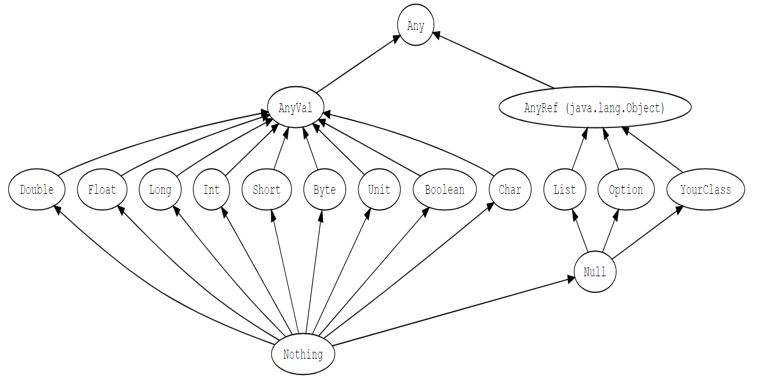
\includegraphics[width=1\textwidth]{pictures/scala-type-hierarchy.jpg}
  \caption{Хијерархија Скала типова}
  \label{fig:scala_types_hier}
\end{figure}

\section{Скала колекције}
\label{sec:scala_coll}

Скала поседује велики број уграђених колекција, мутабилних и имутабилних. Неке од њих су низови, листе, скупови и мапе.

\subsection{Низови}
\label{subsec:scala_arrays}

Скала низ (енг. \textit{array}) је мутабилна структура која представља низ података. Мутабилна је у смислу да се вредности елемената у низу могу мењати, док је број елемената фиксан. Сваки низ садржи елементе једног типа и може се креирати навођењем иницијалних елемената или његове дужине. Уколико се наведе дужина, сви елементи ће бити иницијализовани на подразумевану вредност жељеног типа. \cite{scala_prog}

\begin{lstlisting}[language=Scala, caption={Инстанцирање низа у Скали}, label={lst:scala_coll_array_example}]
scala> val a1 = Array(1, 2, 3)
val a1: Array[Int] = Array(1, 2, 3)

scala> val a2 = new Array[Int](3)
val a2: Array[Int] = Array(0, 0, 0)
\end{lstlisting}

У претходном примеру се у другом случају инстанцира нова класа коришћењем наредбе \textit{new} док у првом то није случај. Разлог је тај што се у првом случају позива метод \textit{apply()} који креира инстанцу низа. Поред тога, у првом случају је Скала компајлер аутоматски закључио тип низа на основу прослеђених елемената, док је у другом тип морао бити експлицитно назначен. \cite{scala_prog}

Елементу низа се приступа слично као у Јави, са тим што се уместо угластих заграда користе обичне. На сличан начин се извршава и мењање једног елемента.

\begin{lstlisting}[language=Scala, caption={Приступ и измена елемента низа}, label={lst:scala_coll_array_get_set}]
scala> val a = Array(1, 2, 3)
val a: Array[Int] = Array(1, 2, 3)

scala> a(0)
val res0: Int = 1

scala> a(0) = 100

scala> a
val res1: Array[Int] = Array(100, 2, 3)
\end{lstlisting}

\subsection{Листе}
\label{subsec:scala_lists}

Скала листе представљају имутабилну колекцију елемената истог типа. Разлика листе у Скали у односу на Јавину је та што је Скала листа увек имутабилна, док Јава листа може бити мутабилна. 

Инстанцира се навођењем елемената. Приступ елементу листе се извршава на исти начин као и у случају низа. Пошто су листе имутабилне, измена вредности елемената није дозвољена. \cite{scala_prog}

\begin{lstlisting}[language=Scala, caption={Пример Скала листе}, label={lst:scala_coll_lists_example}]
scala> val l = List("a", "b", "c")
val l: List[String] = List(a, b, c)

scala> l(0)
val res0: String = a

scala> l(0) = "try"
       ^
       error: value update is not a member of List[String]
       did you mean updated?
\end{lstlisting}

Спајање листи се извршава оператором $:::$. Приликом позива овог оператора се не извршава додавање елемената једне листе на другу, већ је резултат нова листа. Овај метод се може користити и за спајање више од две листе. \cite{scala_prog}

\begin{lstlisting}[language=Scala, caption={Спајање листи}, label={lst:scala_coll_lists_new_list}]
scala> val l1 = List(1, 2, 3)
val l1: List[Int] = List(1, 2, 3)

scala> val l2 = List(4, 5, 6)
val l2: List[Int] = List(4, 5, 6)

scala> val l3 = List(7, 8, 9)
val l3: List[Int] = List(7, 8, 9)

scala> l1 ::: l2 ::: l3
val res0: List[Int] = List(1, 2, 3, 4, 5, 6, 7, 8, 9)
\end{lstlisting}

Нове листе се могу инстанцирати и коришћењем оператора $::$, који као аргументе прима елемент и листу истог типа од којих конструише нову листу где елемент додаје на почетак листе.

\begin{lstlisting}[language=Scala, caption={Пример оператора ::}, label={lst:scala_coll_lists_head_op}]
scala> val l = List(1, 2, 3)
val l: List[Int] = List(1, 2, 3)

scala> 10 :: l
val res0: List[Int] = List(10, 1, 2, 3)
\end{lstlisting}

Коришћењем овог оператора се може извршити надовезивање елемената на празну листу (пример \ref{lst:scala_coll_lists_head_op_nill}). У Скали се празна листа означава кључном речи \textit{Nil}.

\begin{lstlisting}[language=Scala, caption={Додавање елемената на празну листу}, label={lst:scala_coll_lists_head_op_nill}]
scala> val l = 1 :: 2 :: 3 :: 4 :: Nil
val l: List[Int] = List(1, 2, 3, 4)
\end{lstlisting}

\subsection{Н-торке}
\label{subsec:scala_tuple}

Имутабилна колекција која садржи елементе различитог типа се назива н-торка (енг. \textit{Tuple}). Ова структура података се може користити када је потребно вратити више различитих вредности функције. \textit{Tuple} се инстанцира навођењем елемената између заграда. Елементу се приступа оператором \_Х где је \textit{Х} редни број елемента унутар н-торке. \cite{scala_prog}

\begin{lstlisting}[language=Scala, caption={Н-торка у Скали}, label={lst:scala_coll_tuple_example}]
scala> val t = (1, "string123", Array(1, 2, 3))
val t: (Int, String, Array[Int]) = (1,string123,Array(1, 2, 3))

scala> t._1
val res0: Int = 1

scala> t._3
val res1: Array[Int] = Array(1, 2, 3)
\end{lstlisting}

\subsection{Скупови}
\label{subsec:scala_sets}

Скуп је колекција за коју важи да садржи елементе истог типа, са тим што сваки елемент колекције мора бити јединствен. Постоје две врсте скупова, имутабилни (\textit{collection.immutable.Set}) и мутабилни (\textit{collection.mutable.Set}).

Инстанцирају се на исти начин као и низ, навођењем елемената. Уколико се током навођења наведе неки елемент више од једног пута, не добија се грешка, већ се дупликат аутоматски уклања. Елемент се додаје оператором $+$. Код мутабилних скупова $+$ додаје елемент на постојећи скуп, док код имутабилних производи нови скуп са додатим елементом. \cite{scala_prog}

\begin{lstlisting}[language=Scala, caption={Инстанцирање скупа у Скали}, label={lst:scala_coll_set_example}]
scala> val s = Set(1, 1, 1, 1, 2, 2)
val s: scala.collection.immutable.Set[Int] = Set(1, 2)
\end{lstlisting}

\subsection{Мапе}
\label{subsec:scala_maps}

Мапе су колекције за рад са кључ-вредност паровима. Постоје мутабилне (\textit{collection.mutable.Map}) и имутабилне (\textit{collection.immutable.Map}). Имутабилне су подразумеване и користе се уколико се експлицитно не наведе супротно.

Дефинишу се навођењем низа кључ-вредност парова, раздвојених знаком $->$. Сви кључеви и све вредности међусобно морају бити истог типа. Приступ вредностима се врши преко назива кључа, методом $()$.

\begin{lstlisting}[language=Scala, caption={Мапе у Скали}, label={lst:scala_app_maps_example}]
scala> val m1 = Map("k1" -> "v1", "k2" -> "v2")
val m1: scala.collection.Map[String,String] = Map(k1 -> v1, k2 -> v2)

scala> m1("k1")
val res0: String = v1

scala> val m2 = Map(1 -> Array(1, 2), 2 -> Array(3, 4))
val m2: scala.collection.Map[Int,Array[Int]] = Map(1 -> Array(1, 2), 2 -> Array(3, 4))

scala> m2(1)
val res1: Array[Int] = Array(1, 2)
\end{lstlisting}

Разлика између мутабилних и имутабилних мапа је та што је код мутабилних могуће изменити број елемената, као и саме елементе, док имутабилна мапа то не подржава.

\begin{lstlisting}[language=Scala, caption={Измена и додавање елемента код мутабилних и имутабилних мапа}, label={lst:scala_coll_maps_mutable_immutable}]
// mutable map
scala> val mutableM = mutable.Map("k1" -> "v1")
val mutableM: scala.collection.mutable.Map[String,String] = HashMap(k1 -> v1)

scala> mutableM("k1") = "vred1"

scala> mutableM("k2") = "vred2"

scala> mutableM
val res0: scala.collection.mutable.Map[String,String] = HashMap(k1 -> vred1, k2 -> vred2)

// immutable map
scala> val immutableM = Map("k1" -> "v1")
val immutableM: scala.collection.Map[String,String] = Map(k1 -> v1)

scala> immutableM("k1") = "vred1"
       ^
       error: value update is not a member of scala.collection.Map[String,String]

scala> immutableM("k2") = "vred2"
       ^
       error: value update is not a member of scala.collection.Map[String,String]

\end{lstlisting}

\section{Поклапање образаца}
\label{sec:scala_patt_match}

Поклапање образаца (енг. \textit{pattern matching}) је честа карактеристика функционалних језика. Слична је наредби \textit{switch} из Јаве, али нуди више могућности од ње. Састоји се од селектора, који представља израз или променљиву, кључне речи \textit{match} и низа случајева унутар витичастих заграда. Сваки случај се састоји од знака $=>$ који се налази између вредности са којом се селектор поклапа и кључне речи \textit{case} са леве стране и израза који ће бити резултат поклапања са десне. \cite{scala_prog}

\begin{lstlisting}[language=Scala, caption={Поклапање образаца у Скали}, label={lst:scala_coll_patt_match}]
selector match {
	case value1 => result1
	case value2 => result2
	case value3 => result3
	...
}
\end{lstlisting}

Разлике између ове нарeдбе и Јавине наредбе \textit{switch} су:

\begin{itemize} 
\item \textit{match} наредба увек резултује неком вредношћу;
\item Када се пронађе одговарајућа вредност, друге вредности након ње се не разматрају. Није потребно користити наредбу \textit{break};
\item Уколико ниједна вредност не одговара селектору, појављује се \textit{MatchError}. То значи да увек треба покрити све могуће вредности селектора.
\end{itemize}

\subsection{Примери коришћења}
\label{subsec:scala_match_exaples}

Поклапање образаца је веома моћан механизам и користи се у великом броју случајева. Један од њих је поклапање константи:

\begin{lstlisting}[language=Scala, caption={Поклапање константи}, label={lst:scala_patt_match_match_const_example}]
scala> def describe(x: Any) = x match {
     | case 5 => "five"
     | case true => "truth"
     | case "hello" => "hi!"
     | case Nil => "the empty list"
     | case _ => "something else"
     | }
     
scala> describe(5)
val res1: String = five

scala> describe(Nil)
val res2: String = the empty list

scala> describe(1001)
val res3: String = something else
\end{lstlisting}

У претходном примеру се у последњем случају користи ознака $\_$. Назива се џокер (енг. \textit{wildcard}) и поклапа се са било којом вредношћу селектора.

\begin{lstlisting}[language=Scala, caption={Џокер у поклапању образаца}, label={lst:scala_patt_match_wildcard}]
scala> def describe(x: Int) = x match {
     | case 10 => "x je 10"
     | case _ => "x nije 10"
     | }
def describe(x: Int): String

scala> describe(10)
val res1: String = x je 10

scala> describe(100)
val res2: String = x nije 10

scala> describe(-100)
val res3: String = x nije 10
\end{lstlisting}

Поклапање образаца се користи и за поклапање променљивих. У примеру \ref{lst:scala_patt_match_variable_match_example} променљива \textit{something} одговара било којој вредности селектора, слично као џокер, али се преко ње та вредност преноси са десне стране ознаке $=>$. \cite{scala_prog}

\begin{lstlisting}[language=Scala, caption={Поклапање променљивих}, label={lst:scala_patt_match_variable_match_example}]
scala> val expr = "some expression"
val expr: String = some expression

scala> expr match {
     | case ""        => print("empty string")
     | case something => print("matched: " + something)
     | }
matched: some expression
\end{lstlisting}

Поред вредности селектора, могуће је поклапати и његов тип, уколико је потребно имплементирати другачије понашање за другачије типове .

\begin{lstlisting}[language=Scala, caption={Поклапање типова}, label={lst:scala_patt_match_types_example}]
scala> trait MyTrait
trait MyTrait

scala> class MyClass_1 extends MyTrait
class MyClass_1

scala> class MyClass_2 extends MyTrait
class MyClass_2

scala> def describe(x: MyTrait) = x match {
     |   case mc1: MyClass_1 => "MyClass_1"
     |   case mc2: MyClass_2 => "MyClass_2"
     |   case _ => "some other class"
     | }
def describe(x: MyTrait): String

scala> describe(new MyClass_1)
val res1: String = MyClass_1

scala> describe(new MyClass_2)
val res2: String = MyClass_2
\end{lstlisting}

Могуће је комбиновати претходне примере и извршити поклапања типова и променљивих уз помоћ једног поклапања образаца. Пример \ref{lst:scala_patt_match_generalSize} приказује функцију \textit{generalSize(x: Any)} која се понаша другачије у односу на то ког типа је њен аргумент. \cite{scala_prog}

\begin{lstlisting}[language=Scala, caption={Пример поклапања типова и променљивих}, label={lst:scala_patt_match_generalSize}]
scala> def generalSize(x: Any) = x match {
     |   case s: String => s.length
     |   case m: Map[_, _] => m.size
     |   case _ => -1
     |  }
def generalSize(x: Any): Int

scala> generalSize("some string")
val res1: Int = 11

scala> generalSize(12)
val res2: Int = -1
\end{lstlisting}

Поклапање конструктора се користи када је потребно извршити поклапање класа које наслеђују заједничку класу. 

\begin{lstlisting}[language=Scala, caption={Поклапање конструктора}, label={lst:scala_patt_match_constr_match_example}]
scala> abstract class Animal
     | case class Mammal(name: String) extends Animal
     | case class Bird(name: String) extends Animal
class Animal
class Mammal
class Bird

scala> def caseClassesPatternMatching(animal: Animal) = animal match {
     |  case Mammal(name) => s"I'm a $name, a mammal"
     |  case Bird(name) => s"I'm a $name, a bird"
     |  case _ => "I'm an unknown animal"
     |}
def caseClassesPatternMatching(animal: Animal): String
\end{lstlisting}

%\section{Optional и Either}
%\label{sec:scala_opt_eith}=
%optional i either tipovi

%\section{Implicit vred}
%\label{sec:scala_impl_vals}
%implicits
%if requested

\chapter{Дистрибуирана обрада података}
\label{chp:dist_sis}

У последњих неколико година се генерише огромна количина података \cite{volume_data}. Друштвене мреже, видео садржај и куповина преко интернета на дневном нивоу производе петабајте података, а у будућности се очекује пораст тог тренда. Како је често проблем обрадити огромне количине података на једној машини, индустријски стандард су постали кластери који раде са подацима на дистрибуиран начин.

% да ли овде направити увод у мерне јединице???
\begin{comment}

\begin{center}
\begin{tabular}{|c|c|}
	\hline
 	Мерна јединица меморије & Вредност \\ \hline
	Бит & 0 или 1 \\ \hline
	Бајт & 8 бита \\ \hline 	
 	Килобајт & 1024 бајта \\ \hline
 	Мегабајт & 1024 килобајта \\ \hline
 	Гигабајт & 1024 мегабајта \\ \hline
 	Терабајт & 1024 гигабајта \\ \hline
 	Петабајт & 1024 терабајта \\ \hline
 	Егзабајт & 1024 петабајта \\ \hline
\end{tabular}
\end{center}

\end{comment}

% подаци су свуда око нас бла бла бла???

\section{Доба података} % подаци данас?
\label{sec:dist_motivacija}

Према истраживању \cite{volume_data} приказаном на једном од водећих интернет платформи за податке који се користе у пословању, \textit{Statista}, количина података која се производи се тренутно може мерити у зетабајтима (милионима петабајта). Исто истраживање приказује да ће се наредних година тај број удвостручити. Приказ пораста тренда генерисања података је приказан на слици \ref{fig:kolicina_podataka}.

Корист података је огромна и велики број индустрија и компанија их користи на разне начине, од побољшања искуства корисника који користе њихове услуге, до разних предвиђања у пословању. Из тих разлога се доста улаже у складиштење, обраду, истраживање и анализу података. Подаци су се раније, док још увек нису генерисани у количинама у којима се то дешава данас, обрађивали на појединачним машинама, али се убрзо испоставило да такав приступ има своја ограничења.

\begin{figure}[!ht]
  \centering
  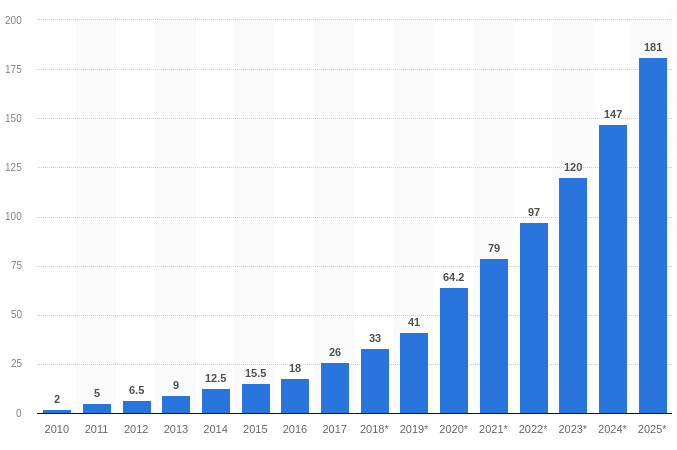
\includegraphics[width=0.8\textwidth]{pictures/Total_data_volume_worldwide_2010_2025_statista.png}
  \caption{Kоличина података по години у зетабајтима \cite{volume_data}}
  \label{fig:kolicina_podataka}
\end{figure}

\section{Скалирање система}
\label{sec:skaliranje}

У контексту система, скалирање означава могућност система да се прилагоди количини података који се уз помоћ њега обрађују. Постоје два начина скалирања уређаја који врше обраду података (слика \ref{fig:skaliranje}). Први начин је вертикално скалирање (енг. \textit{vertical scaling}) или \textit{scale-up} \cite{hadoop_beginner}. У овом приступу се унапређује једна машина, на пример, додавањем веће количине меморије или појачавањем снаге процесора. Предност овог приступа је што се након унапређења машине не мора мењати логика апликација које се на њој извршавају. Али негативна особина је што постоји ограничење до ког се машина може унапредити, па стога постоји и ограничење у количини података које она може обрадити. Такође, у случају грешке, цео систем престаје са радом, пошто се састоји од само једне машине.

Други приступ је хоризонтално скалирање (енг. \textit{horizontal scaling}) или \textit{scale-out} \cite{hadoop_beginner}. У овом случају се не унапређује једна машнина, већ се, уколико је потребна додатна снага, додаје нова машина у систем. Добра особина овог приступа је што је често јефтиније додати неколико нових машина у систем него унапредити процесор неколико пута на истој машини. Још једна веома добра одлика је ефикасност. Када постоји неколико машина могуће је на свакој од њих обрађивати један део података, што је огромна предност у односу на вертикално скалирање. Међутим, хоризонтално скалирање доноси додатан скуп проблема. Потребно је имплементирати цео систем, омогућити машинама да раде заједно и координисати их, као и обрадити грешке који се могу десити на појединачним машинама. Како су наведене предности значајне, а мане се могу превазићи, данашњи стандард у обради података је хоризонтално скалирање.

\begin{figure}[!ht]
  \centering
  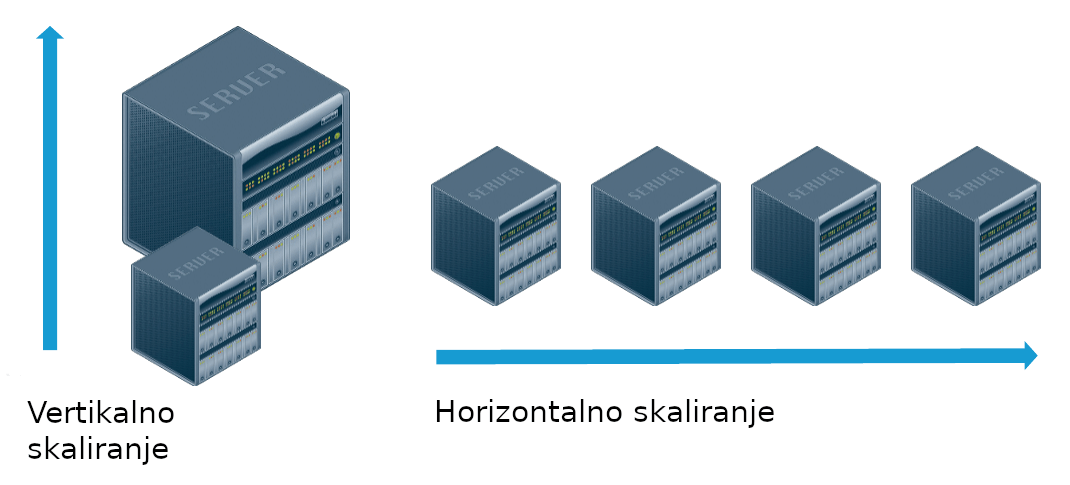
\includegraphics[width=0.9\textwidth]{pictures/scaling.png}
  \caption{Врсте скалирања система}
  \label{fig:skaliranje}
\end{figure}

\section{Организација дистрибуираних система}
\label{sec:scaling_osobine}

У оквиру хоризонталног скалирања свака машина у систему обрађује један део података и на тај начин доприноси коначном резултату, због чега машине морају да комуницирају једна са другом \cite{hadoop_beginner}. Поред тога, могуће је да постоје подаци који су потребни свим машинама у систему, што може довести до такмичења уређаја за приступ тим подацима. Уколико се подаци налазе на само једној машини у систему, све друге машине ће јој приступити, тако да су могућности система у том случају ограничене могућностима те једне машине којој све остале приступају. Поред тога, на тој машини се може догодити некакав проблем због ког она престане да функционише, што би изазвало престанак рада целог система.

Да би се потенцијални проблеми избегли, систем треба да функционише тако да уређаји који су у њему раде независно од других уређаја истог система, као и да престанак рада једне машине не утиче на систем у целини. Другим речима, треба направити систем који очекује да се фаталне грешке дешавају. 

У оваквим системима акценат је на софтверу, а не на хардверу и идеја је да се систем може направити од уређаја који су релативно јефтини и масовно доступни \cite{hadoop_beginner}. Такође, циљ је да се избегава премештање података међу уређајима, па се подаци, уколико је то могуће, обрађују на машини на којој се налазе.

\section{Систем \textit{Hadoop}}
\label{sec:hadoop}

Први успешан систем који поседује претходно наведене карактеристике је развила компанија \textit{Google} која је 2003. године објавила научни рад на ту тему \cite{gfs}. У раду је представљен дистрибуирани фајл систем, назван \textit{Google file system} или скраћено \textit{GFS}. Систем је написан у програмском језику \textit{C++}. Намена овог система је да се користи за складиштење великих количина података. Већ следеће године, \textit{Google} је објавио нови научни рад о парадигми за ефикасну обраду велике количине података на кластеру \cite{gmr}. Парадигма је названа \textit{MapReduce} и њена намена је да се користи за обраду података складиштених у \textit{GFS}-у.

Недуго након тога, уз помоћ научних радова компаније \textit{Google}, настао је пројекат отвореног кода (енг. \textit{оpen source}) назван \textit{Hadoop} са идејом да имплементира карактеристике које поседују \textit{Google}-ови \textit{GFS} и \textit{MapReduce} и да се као такав користи за складиштење и ефикасну обраду падатака на кластеру сачињеном од релативно јефтиних машина \cite{hadoop_beginner}. Највећи делови \textit{Hadoop} система су \textit{Hadoop distributed file system}, скраћено \textit{HDFS}, и парадигма \textit{MapReduce} који су заправо јавно доступни еквиваленти \textit{Google}-ових технологија. Њихови логои су приказани на слици \ref{fig:hdfs_mr_logo}.

Укратко, \textit{HDFS} је фајл систем који користи хоризонтално скалирање машина за складиштење огромних количина података \cite{hadoop_beginner}. Због боље поузданости користи репликацију, где се сваки фајл копира неколико пута и онда се те копије чувају на различитим уређајима у систему.

\textit{MapReduce} је парадигма за обраду података, која се састоји из два дела названа \textit{Мap} и \textit{Reduce}, по којима је и добила име \cite{hadoop_beginner}. Улога \textit{Map} дела је да чита података из \textit{HDFS}-а у деловима и трансформише их, док \textit{Reduce} прикупља резултате обраде \textit{Map} фазе и спаја их у један. Обрада се извршава на истим машинама \textit{HDFS}-а на којима се подаци и налазе, чиме се избегава њихово премештање на неку другу машину.

\begin{figure}[!ht]
  \centering
  
\includegraphics[width=0.8\textwidth]{pictures/hdfs_mr_logo.png}
  \caption{Логои \textit{HDFS}-а и \textit{MapReduce}-а}
  \label{fig:hdfs_mr_logo}
\end{figure}

Поред поменуте две компоненте, постоји и трећа, а то су \textit{HDFS} апликације \cite{hadoop_learning}. Оне се надовезују на \textit{HDFS} и \textit{MapReduce} тако што их користе за, редом, складиштење и обраду података. Најпознатије су \textit{Apache Hive} \cite{apache_hive} и \textit{Apache Pig} \cite{apache_pig}, али поред њих постоје и многе друге, само мање заступљене. На слици \ref{fig:hadoop_aplikacije} су приказане компоненте \textit{Hadoop}-а.

\begin{figure}[!ht]
  \centering
  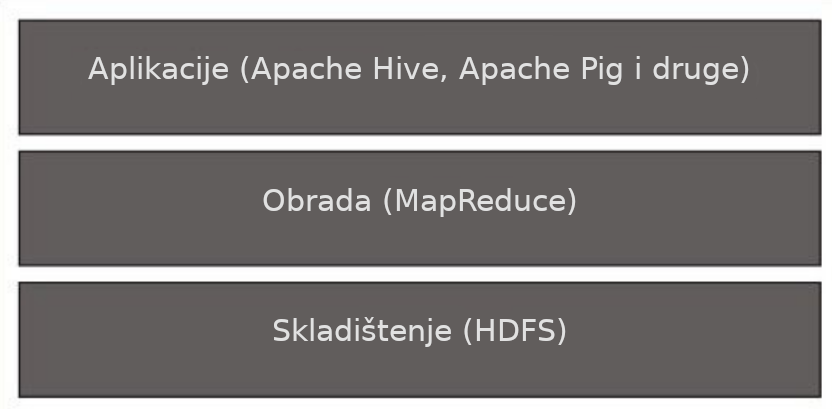
\includegraphics[width=0.7\textwidth]{pictures/hadoop_apps.png}
  \caption{Упрошћен приказ \textit{Hadoop}-а}
  \label{fig:hadoop_aplikacije}
\end{figure}

\section{Дистрибуирани фајл систем \textit{HDFS}}
\label{sec:hdfs}

\textit{HDFS}, скраћено од \textit{Hadoop distributed file system} је дистрибуирани систем, што значи да складишти податке на више машина које ће се у даљем тексту звати чворови (енг. \textit{nodes}). Скуп машина које раде заједно на такав начин да се могу посматрати као једна целина се назива кластер (енг. \textit{cluster}). 

\subsection{Структура \textit{HDFS}-а}
\label{subsec:hdfs_nodes}

Постоје две врсте чворова, именски чвор (енг. \textit{name node}) и чвор података (енг. \textit{data node}). Функционишу по водећи-зависни (енг. \textit{master-slave}) архитектури, где именски чвор има улогу водећег. Чворови су приказани на слици \ref{fig:hadoop_nodovi}.

Унутар \textit{HDFS} система се налази један примарни именски чвор чија је улога да управља фајл системом и да регулише приступ подацима који се налазе на њему \cite{hadoop_arch_guide}. Он садржи информације о фајловима, као што су, између осталих, име, локација у систему где се фајл налази, последњи датум измене фајла као и правила приступа. Поред примарног, \textit{HDFS} може имати и неколико секундарних именских чворова који представљају резервне копије.

Чворови података имају улогу да складиште фајлове система \cite{hadoop_arch_guide}. Поред тога, на овим чворовима се извршава обрада података. Чворови података су задужени за операције над фајловима као што су читање, мењање и брисање. Они ће извршити неку од тих операција само када им именски чвор то нареди.

\begin{figure}[!ht]
  \centering
  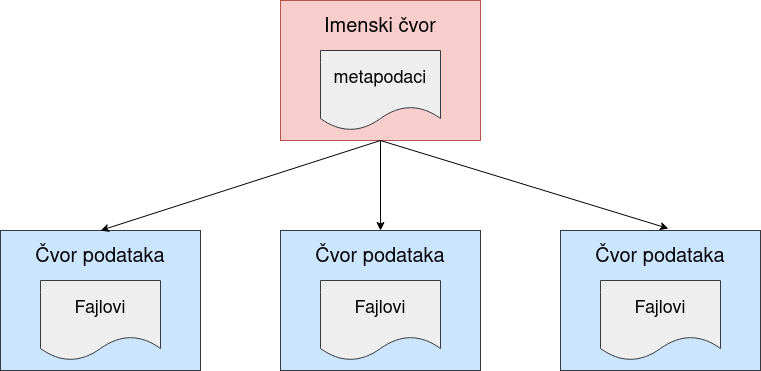
\includegraphics[width=0.92\textwidth]{pictures/node_types.png}
  \caption{Врсте чворова у \textit{HDFS}-у}
  \label{fig:hadoop_nodovi}
\end{figure}

Уколико апликација жели да приступи \textit{HDFS}-у, она ће прво комуницирати са именским чвором и од њега затражити фајлове који јој требају. Након тога, именски чвор проверава да ли та апликација поседује потребне дозволе за приступ тим фајловима и ако их она има, послаће јој њихову локацију у фајл систему. Након тога се може извршити жељени приступ. 

\subsection{Основне карактеристике \textit{HDFS}-а}
\label{subsec:hdfs_osobine}

Сваки фајл у \textit{HDFS}-у је подељен на делове који се називају блокови чија је величина обично 128 мегабајта \cite{hadoop_arch_guide}. Блокови се често не налазе на истим чворовима у систему, што значи да се један фајл чува на неколико физички раздвојених машина. Ту може да настане проблем због тога што једна од тих машина може да се поквари и због тога престане са радом. У том сличају ће сви блокови складиштени на тој машини нестати. Да би се губљење фајлова избегло, \textit{HDFS} сваки блок реплицира неколико пута и након тога оригинални блок и његове реплике распоређује по систему. Ако један од блокова фајла неочекивано нестане, увек је могуће приступити једној од његових реплика. Генерисане реплике се чувају на чворовима података, док се информације о томе ком фајлу реплике припадају налазе на именском чвору.

Блок ће се увек реплицирати одређен, фиксиран, број пута. Чворови података повремено шаљу сигнале именском чвору о доступности реплика. На тај начин ће именски чвор увек имати информацију о томе колико је пута сваки блок реплициран у систему и на основу тога може да, уколико тај број падне испод неке задовољавајуће вредности, направи нове реплике тог блока \cite{hadoop_arch_guide}.

\textit{HDFS} је конструисан тако да може да настави са радом у случају фаталних грешака на чворовима података. Међутим, могућа је појава грешака и на именском чвору и те грешке могу довести до пада целокупног система. Такви проблеми се решавају чувањем резервних копија именског чвора и због њих се у случају престанка његовог рада не губе информације. Резервне копије се праве у одређеним временским интервалима да би подаци на њима били ажурни. Резервне копије и репликација су битне за целокупну робусност система, односно поузданости података. Концепти \textit{HDFS}-а су приказани на слици \ref{fig:hadoop_sistem}.

\begin{figure}[!ht]
  \centering
  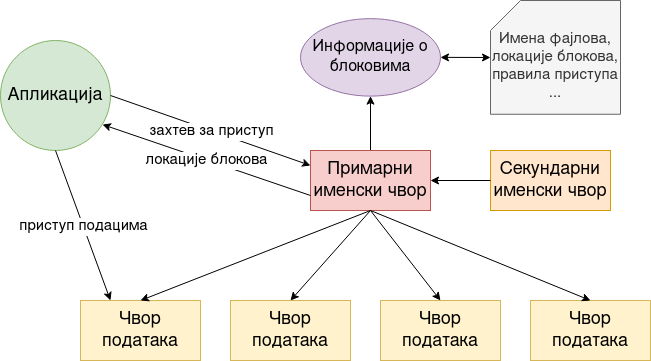
\includegraphics[width=1\textwidth]{pictures/hdfs_components_basic.png}
  \caption{Основне \textit{HDFS} компоненте}
  \label{fig:hadoop_sistem}
\end{figure}

\textit{HDFS} је систем за кога важи \textit{пиши једном, читај више пута} (енг. \textit{write-once, read-many)}. Када се фајл постави унутар \textit{HDFS}-а више се не може мењати \cite{hadoop_beginner}. Уколико се фајл мора изменити долази до креирања новог фајла који замењује стари. Иако такав приступ није ефикасан, апликације које обрађују велике количине података се обично заснивају на томе да се подаци не мењају, па се очекује да за променама неће бити потребе или ће такви случајеви бити ретки. Такође, још једна од особина \textit{HDFS}-а је да има добре перформансе у случајевима када је потребан велики проток података, на пример у случају читања великих фајлова.

% https://www.quora.com/Is-HDFS-an-append-only-file-system-Then-how-do-people-modify-the-files-stored-on-HDFS.

\section{Парадигма \textit{MapReduce}}
\label{sec:mr}

\textit{МapRreduce} је парадигма која се користи за обраду података који су складиштени у \textit{HDFS}-у \cite{hadoop_beginner}. Користи подели и завладај (енг. \textit{divide and conquer}) приступ приликом обраде тако да више машина паралелно обрађује један део података.

Парадигма је заснована на концептима функционалног програмирања и функцијама које се често користе у обради низова и листи. Те фунције су \textit{map} и \textit{reduce}. Прва од постојеће листе креира нову тако што на сваки елемент листе примени неку фунцију и од њега направи нови елемент. Друга од целе листе производи једну вредност. На истим принципима фунционише и \textit{MapReduce}.

\textit{MapReduce} обрађује податке у неколико фаза \cite{hadoop_learning}. Прво, подаци се читају из \textit{HDFS}-а и након тога прослеђују машинама које се зову мапери (енг. \textit{mappers}). Те машине паралелно производе скуп привремених података који се након тога распоређују, сортирају и шаљу машинама које се зову редјусери (енг. \textit{reducers}). Фаза која распоређује податке се назива фаза мешања и сортирања (енг. \textit{shuffle and sort}). Задатак редјусера је да приме подскуп података и да паралелно произведу једну вредност од истих. На самом крају се резултат свих редјусера комбинује и добија се резултат читавог \textit{MapReduce} процеса, другачије названог и \textit{MapReduce} задатак (енг. \textit{task}). Могуће је, уланчавањем, комбиновати \textit{MapReduce} задатке, тако да излаз из једног буде улаз у други. Скуп повезаних \textit{MapReduce} задатака се назива \textit{MapReduce} апликација.

\subsection{\textit{MapReduce} из аспекта функција}
\label{subsec:mr_funck_asp}

Из аспекта функција, \textit{map} и \textit{reduce} фазе се могу посматрати на следећи начин. Подразумевани формат је \textit{(кључ, вредност)} за који ће се због једноставности користити ознака \textit{(k, v)}. Током \textit{map} фазе подаци се читају из \textit{HDFS}-а и деле на делове на које се паралелно примењује функција \textit{map} дефинисана од стране програмера. Паралелизам се постиже тако што се сваки део обрађује на засебној машини, маперу. Фаза \textit{map} као улаз прима \textit{(k, v)} паровe и производи листу истог формата \cite{hadoop_learning}.

$$ (k_1, v_1) \rightarrow map(k_1, v_1) \rightarrow list(k_2, v_2) $$

Након тога се листе генерисане од мапера групишу тако што се за сваки кључ прави једна група коју ће обрадити један редјусер. Овај део обраде је \textit{shuffle and sort}. 

$$ list(k_2, v_2) \rightarrow shuffleAndSort(k_2, v_2) \rightarrow k_2, list(v_2) $$

У последњој фази се на сваку од креираних група примењује функција \textit{reduce} која производи једну вредност за сваку групу \cite{hadoop_learning}. Овај процес је паралелизован и није могуће да се две групе података са различитим кључевима обрађују на истој машини у истом тренутку. Фаза \textit{Reduce} прима кључ и листу вредности које му одговарају и као резултат производи једну вредност формата \textit{(k, v)}.

$$ k_2, list(v_2) \rightarrow reduce(k_2, list(v_2)) \rightarrow (k_3, v_3) $$

Коначан резултат се добија комбиновањем резултата свих редјусера и може се уписати у \textit{HDFS} или се искористити као улаз у други \textit{MapReduce} задатак. У \textit{MapReduce} апликацијама задатак програмера је да опише како ће се извршавати \textit{map} и \textit{reduce} фазе, док ће се \textit{Hadoop} систем побринути за све остало: читање података, сортирање, паралелизацију, координацију и извршавање послова \cite{hadoop_beginner}.

Пример \textit{MapReduce} апликације је приказан на слици \ref{fig:map_reduce} где је представљен процес пребројавања броја појављивања сваке речи у тексту. У приказаном примеру је улаз у мапере форматиран тако да је редни број линије фајла кључ, док је текст линије вредност. Улога мапера је да поделе текст на речи и да од њих направе листу парова формата \textit{(реч, 1)}. Након тога се парови који имају исту реч премештају на засебне редјусере који израчунавају колико пута се у почетном скупу појављује свака реч, сумирањем јединица.

\begin{figure}[!ht]
  \centering
  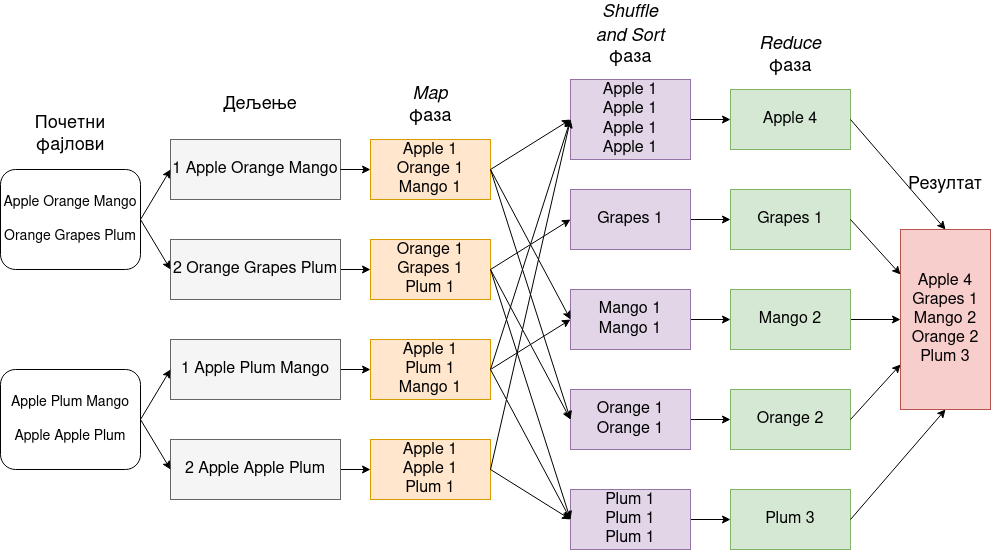
\includegraphics[width=1\textwidth]{pictures/mr_example_wordcount.png}
  \caption{Пример \textit{MapReduce} апликације}
  \label{fig:map_reduce}
\end{figure}

% Oва парадигма je направљена да ради за податке у \textit{(кључ, вредност)} формату, а не за податке који имају дефинисану шему. Пример података који имају шему би биле табеле у релационим моделима. \cite{hadoop_beginner}

\subsection{Недостаци \textit{MapReduce} парадигме}
\label{subsec:nedost_mr}

\textit{MapReduce} апликација се састоји од ланца \textit{MapReduce} послова, таквих да излаз једног посла представља улаз у други (слика \ref{fig:mr_app_example}). Међутим, такав приступ има цену, а то је да се излаз генерисан од стране једног \textit{MapReduce} посла чува унутар \textit{HDFS}-а, одакле му приступају други \textit{MapReduce} послови којима је тај излаз потребан \cite{hadoop_learning}. Другим речима, међурезултати послова се чувају на диску, што ствара додатне улазно/излазне операције и тиме успорава извршавање целокупне апликације. Поред тога, унутар \textit{MapReduce} парадигме не постоји аутоматски начин да се послови заједно оптимизују, на пример комбиновањем, већ је за то задужен програмер.

\begin{figure}[!ht]
  \centering
  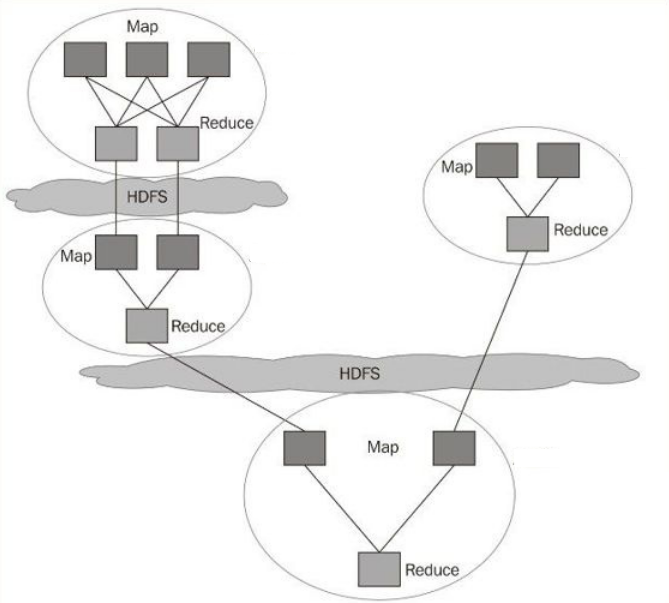
\includegraphics[width=0.9\textwidth]{pictures/mr_app.png}
  \caption{Пример ланца \textit{MapReduce} послова}
  \label{fig:mr_app_example}
\end{figure}

Због поменутих недостатака се \textit{MapReduce} парадигма у данашње време ретко користи. Потиснута је од стране других технологија и алата, међу којима је и \textit{Apache Spark}  (поглавље \ref{chp:spark}).

\section{Преговарач ресурса \textit{Apache Yarn}}
\label{sec:yarn}

У првој верзији \textit{Hadoop}-а, \textit{MapReduce} је поред обраде великих количина података, за шта је примарно и намењен, имао додатне задатке, а то су заказивање \textit{MapReduce} задатака и алокација и управљање ресурсима који су \textit{MapReduce} апликацији потребни \cite{hadoop_learning}. Таква архитектура је знатно отежавала конструкцију апликација које користе \textit{MapReduce}, па су због тога, у другој верзији \textit{Hadoop}-а, одговорности \textit{MapReduce}-а раздвојене. \textit{MapReduce} је постао алат искључиво за обраду података, док је управљање ресурсима предато новој апликацији, са идејом да је \textit{MapReduce} током извршавања користи.

Резултат је менаџер ресурса (енг. \textit{resource manager}) отвореног кода назван \textit{Yarn} \cite{yarn} или \textit{yet another resource negotiator}. Његова улога је да распоређује задатке апликација које користе \textit{Hadoop}, али и да управља ресурсима који су тим апликацијама потребни  \cite{hadoop_learning}. Конструисан је да не буде специфичан само за \textit{MapReduce}, већ пружа интерфејс ка \textit{Hadoop}-у разним апликацијама међу којима је и \textit{Apache Spark}. Разлика у архитектури у различитим верзијама \textit{Hadoop}-а је приказана на слици \ref{fig:yarn_hadoop_versions}.

\begin{figure}[!ht]
  \centering
  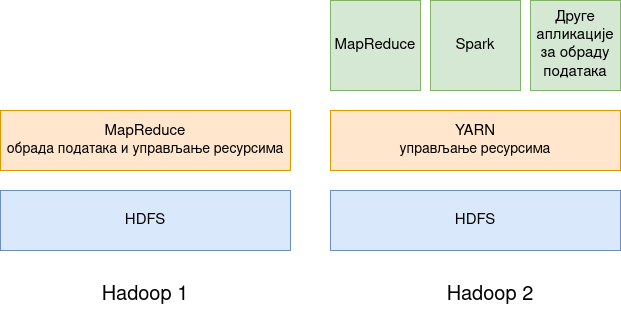
\includegraphics[width=1\textwidth]{pictures/mr_yarn_hadoop_versions.png}
  \caption{Разлика у архитектури између \textit{Hadoop} верзија}
  \label{fig:yarn_hadoop_versions}
\end{figure}

\subsection{Архитектура \textit{Yarn}-а}
\label{subsec:yern_arch}

Улога \textit{Yarn}-а је искључиво да распореди извршавање задатака на кластеру и обезбеди им ресурсе потребне за њихово извршавање \cite{hadoop_learning}. Све остало, попут надгледања система, праћења прогреса апликација, обраде грешака и сличног, је имплементирано у коду апликације која га користи. % Разлог томе је идеја да \textit{Yarn} буде што је више могуће самосталан, да би различите врсте апликација могле да га користе.

Састоји је од две главне компоненте, менаџера ресурса (енг. \textit{resource manager}) и од менаџера чворова (енг. \textit{node manager}) \cite{hadoop_learning}. Улога првог менаџера је да управља ресурсима читавог кластера, док други управља ресурсима машине на којој је покренут. То значи да ће кластер имати један менаџер ресурса и више менаџера чворова, по један за сваку машину у кластеру. Заједно, они управљају контејнерима (енг. \textit{container}), апстракцијом меморије, процесорске снаге и улазно-излазних операција потребних да би се извршио један део апликације на кластеру.

Менаџер ресурса је најбитнија компонента \textit{Yarn}-а и одговоран је за извршавање сваке апликације на кластеру \cite{hadoop_learning}. Састоји се од две компоненте, заказивача (енг. \textit{scheduler}) и менаџера апликације (енг. \textit{application manager}). Прва регулише распоред извршавања апликација, док друга прихвата апликације и преговара о алокацији првог контејнера који им је потребан.

Апликација која се покреће преко \textit{Yarn}-а се састоји из два дела. Први је к\^{o}д који треба извршити на кластеру, док се други зове мастер апликације (енг. \textit{application master}) \cite{hadoop_learning}. Његова улога је да преговара о ресурсима и прати прогрес и статус апликације. \textit{Yarn} нема информацију на који начин је успостављена комуникација између мастера апликације и кода који се извршава. Приказ архитектуре и компоненти \textit{Yarn}-а у случају извршавања две апликације на кластеру је приказан на слици \ref{fig:yarn_ar}.

Процес покретања апликације преко \textit{Yarn}-а се извршава следећим редоследом:

\begin{enumerate}
	\item Клијент пријављује апликацију.
	\item Менаџер ресурса алоцира контејнер на чвору у коме се покреће мастер апликације.
	\item Мастер апликације се региструје код менаџера ресурса.
	\item Мастер апликације преговара о контејнерима са менаџером ресурса. У исто време, заказивач распоређује извршавање делова апликације.
	\item Мастер апликације комунуцира са менаџером чвора о покретању потребних контејнера за извршавање апликације.
	\item К\^{о}д апликације се извршава унутар контејнера.
	\item Клијент преко менаџера ресурса и мастера апликације прати прогрес апликације.
	\item Процес је завршен, мастер апликације се одјављује од менаџера ресурса.
\end{enumerate}

\begin{figure}[!ht]
  \centering
  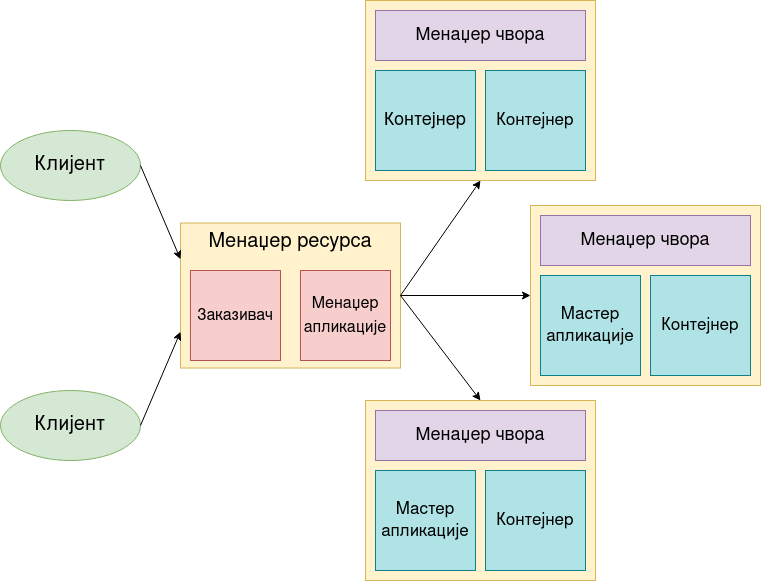
\includegraphics[width=0.93\textwidth]{pictures/yarn_arch.png}
  \caption{Компоненте \textit{Yarn}-а у случају извршавања две апликације}
  \label{fig:yarn_ar}
\end{figure}

%Апликације се, користећи \textit{Yarn}, на кластеру покрећу преко клијента. Када \textit{Yarn} апликација започне са радом, клијент прво комуницира са менаџером ресурса и преко њега захтева иницијални контејнер на коме ће покренути мастер апликације. У већини случајева се мастер апликације покреће унутар једног контејнера у кластеру, исто као што се покреће и к\^{о}д апликације. Након тога почиње комуникација између покренутог мастера апликације и менаџера ресурса. Kомуникација се одвија тако што мастер апликације захтева од менаџера ресурса контејнере који су потребни апликацији и менаџер ресурса након тога шаље податке мастеру апликације о контејнерима које апликација може да користи. Користећи те информације, мастер апликације комуницира са менаџерима чворова који се налазе на истим машинама као и захтевани контејнери и пружа им спецификације о апликацији која треба да буде покренута у тим контејнерима. Након тога, менаџери чворова започињу извршавање апликације. Од овог тренутка, даље понашање апликације зависи од кода те апликације. \cite{hadoop_learning}

\textit{Yarn} има одговорност да омогући правилно извршавање апликацијама које се извршавају на \textit{HDFS}-у па стога мора обрадити грешке које се могу појавити \cite{hadoop_learning}. На пример, могуће је да једна од машина у кластеру престане се радом и тако постане неупотребљива. Када се то деси, менаџер ресурса ће менаџер чвора на тој машини означити мртвим и неће га више разматрати. Исто ће се десити и са контејнерима те машине. Такође, сваки контејнер који почне да користи више ресурса од оних који су му омогућени ће бити уништен, да не би изазивао проблеме другим апликацијама у систему.

\section{Остале компоненте \textit{Hadoop}-а}
\label{sec:ostale_komp_hadupa}

\textit{Hadoop} екосистем чини велики број апликација разних примена које на неки начин користе \textit{HDFS}. Поред самог \textit{HDFS}-а, \textit{MapReduce}-а и \textit{Apache Yarn}-а у њега спадају и \textit{Apache Kafka} \cite{apache_kafka}, апликација за рад са токовима података, \textit{Apache Pig} \cite{apache_pig} и \textit{Apache Hive} \cite{apache_hive}, које се користе за обраду података и имплементиране су коришћењем \textit{MapReduce}-а. Поред њих постоје, на пример,  \textit{Presto} \cite{presto}, \textit{Apache Flume} \cite{apache_flume}, \textit{Apache Zookeeper} \cite{apache_zookeeper} али и многе друге. Приказ малог дела \textit{Hadoop} екосистема је приказан на слици \ref{fig:hadoop_ecosystem}.

\begin{figure}[!ht]
  \centering
  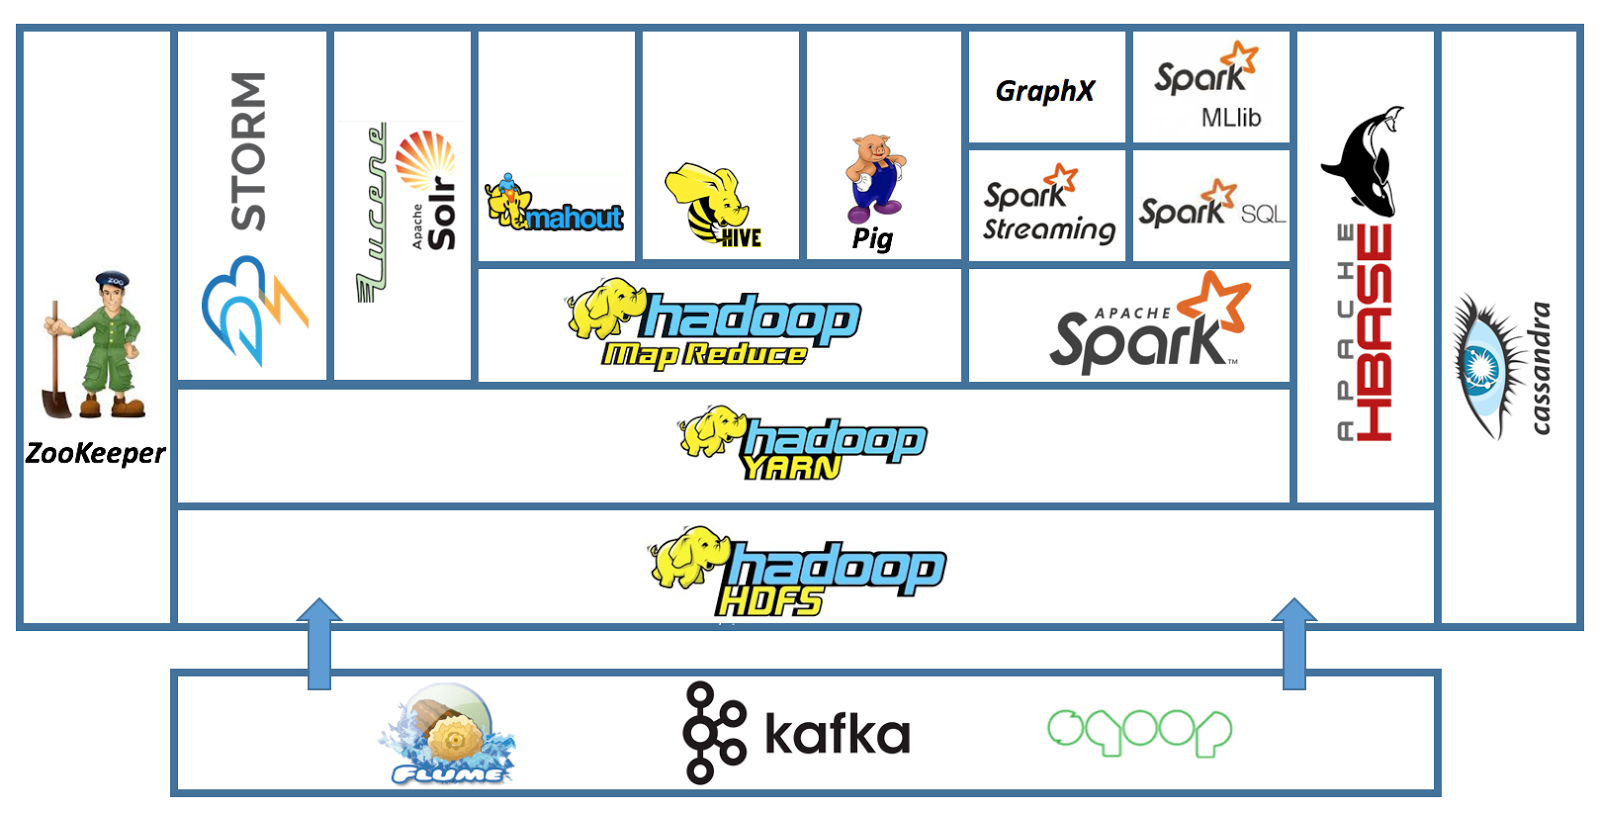
\includegraphics[width=1\textwidth]{pictures/hadoop_ecosystem.png}
  \caption{Део \textit{Hadoop} екосистема}
  \label{fig:hadoop_ecosystem}
\end{figure}

\chapter{Алат \textit{Apache Spark}}
\label{chp:spark}

%Иако је \textit{MapReduce} парадигма обележила почетак доба обраде великих количина података, у данашње време се ретко користи. Примаран разлог томе су недовољно добре перформансе

\textit{Apache Spark} је алат отвореног кода. Настао je 2009. године на универзитету Беркли (енг. \textit{Berkeley}) у Калифорнији. Написан је у програмском језику Скала и конструисан је са идејом да користи концепте функционалног програмирања. Постао је део \textit{Apache} фондације 2013. године. Од тада су избачене три верзије, редом назване, \textit{Spark} 1.0 (2013. године), \textit{Spark} 2.0 (2016. године) и \textit{Spark} 3.0 (2020. године).

Намењен је за дистрибуирану обраду велике количине података али  се поред тога користи и за рад са токовима података (енг. \textit{streaming}), машинско учење и рад са графовима \cite{spark_guide}. Подржан је у програмским језицима \textit{Scala}, \textit{Java}, \textit{Python} и \textit{R}. Иако је намењен за рад над кластерима, може се користити и на једној машини. На слици \ref{fig:spark_kompot} су приказане компоненте \textit{Apache Spark}-а. У овој секцији ће детаљније бити приказане оне које се користе за обраду података.

\begin{figure}[!ht]
  \centering
  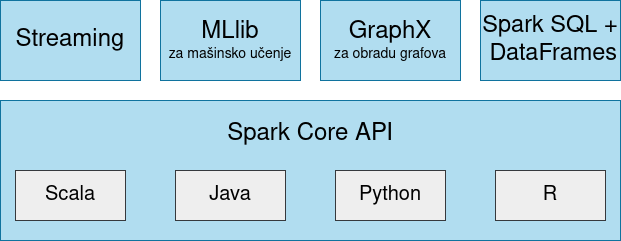
\includegraphics[width=1\textwidth]{pictures/spark_components.png}
  \caption{Компоненте \textit{Apache Spark}-a}
  \label{fig:spark_kompot}
\end{figure}

\section{Архитектура}
\label{sec:spark_arx}

Да би \textit{Spark} могао да приступа кластеру, потребно му је омогућити приступ уз помоћ менаџера ресурса. Иако \textit{Spark} поседује сопствени менаџер ресурса, могу се користити и други, попут \textit{Apache Yarn}-а. Након повезивања је могуће покренути \textit{Spark} апликације на кластеру. 

Свака \textit{Spark} апликација се састоји из једног драјвер процеса (енг. \textit{driver process}) и једног или више извршилац процеса (енг. \textit{executor process}). Драјвер процес је срце \textit{Spark} апликације и има три задужења:

\begin{itemize}
	\item прикупљање информација о апликацији која се извршава;
	\item реаговање на програм апликације и њен унос;
	\item анализирање, распоређивање и планирање послова који се извршавају на извршиоцима.
\end{itemize}

Изрвшиоци имају улогу да извршавају посао који им драјвер процес задаје. Поред тога, задужени су и за пријављивање стања извршавања тог посла драјверу. 

Унутар драјвера постоји одвојен процес назван спарк контекст (енг. \textit{spark context}) \cite{spark_guide}. Његова улога је да дефинише конекцију ка кластеру. Такође се користи и за креирање апстракција \textit{Apache Spark}-а названих \textit{RDD} (поглавље \ref{sec:spark_rdd}). Једноставан приказ архитектуре \textit{Spark}-а је дат на слици \ref{fig:spark_arhtt}.

\begin{figure}[!ht]
  \centering
  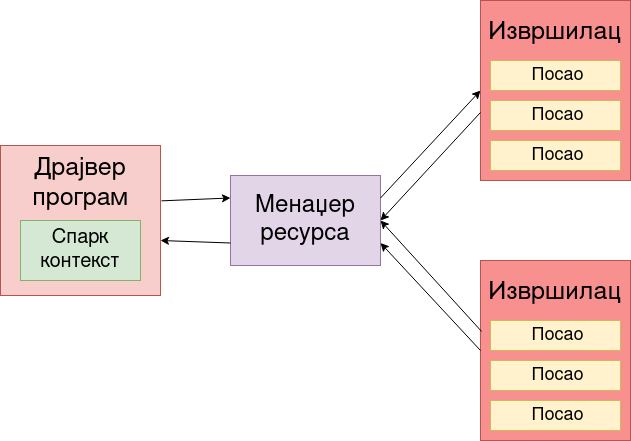
\includegraphics[width=0.90\textwidth]{pictures/spark_arch.png}
  \caption{Архитектура \textit{Apache Spark}-а}
  \label{fig:spark_arhtt}
\end{figure}

Архитектура је заснована на истим концептима, независно од тога да ли се \textit{Spark} покреће у локалном моду, на једној машини, или на кластеру. Једина разлика је у томе што се на кластеру драјвер и извршиоци налазе на различитим машинама, док ће локално бити покренути на истој.

\section{Партиције}
\label{sec:spark_partic}

Да би извршиоци могли паралелно да извршавају операције над подацима, \textit{Spark} податке дели на делове који се називају партиције (енг. \textit{partitions}) \cite{spark_guide}. Партиција је део колекције података који се налази на једној машини кластера. За партиције важи да се једна партиција увек обрађује од стране једног извршиоца, као и да један извршилац, у једном тренутку, обрађује податке тачно једне партиције.

%Свака партиција се обрађује од стране једне машине, па је могуће извршити обраду већег броја партиција у исто време, на различитим машинама, чиме се постиже паралелизам. Такође, једна машина може обрађивати само једну партицију у једном тренутку

% свака партиција се обрађује од стране једне машине, па је могуће извршити обраду већег броја партиција у исто време, чиме се постиже паралелизам.

Уколико су подаци партиционисани само једном партицијом, биће обрађени од стране једног извршиоца у кластеру, независно од тога колико извршилаца постоји. Слично, уколико је креирано више партиција, али постоји само један извршилац, паралелизам неће постојати, због тога што постоји само једна машина која може обрадити податке.

\section{Апстракција података \textit{RDD}}
\label{sec:spark_rdd}

Основна јединица рада у \textit{Spark}-у се назива \textit{RDD}, скраћено од \textit{resilient distributed dataset}, и све операције са подацима се извршавају преко ње. \textit{RDD} је колекција елемената за које важи да су партиционисани по машинама кластера и да се над њима паралелно могу извршавати операције \cite{spark_rdd}. Постоји неколико начина преко којих се \textit{RDD} може креирати:
\begin{itemize}
\item Читањем неког фајла који се налази на фајл систему (обично \textit{HDFS});
\item Од колекција података програмског језика у коме се користи \textit{Spark} (слика \ref{fig:spark_rdd_creation_png}). Процес дељења колекције у партиције се назива паралелизација;
\item Од већ постојећег \textit{RDD}-ја;
\item Кеширањем постојећег \textit{RDD}-ја.
\end{itemize}

\begin{figure}[!ht]
  \centering
  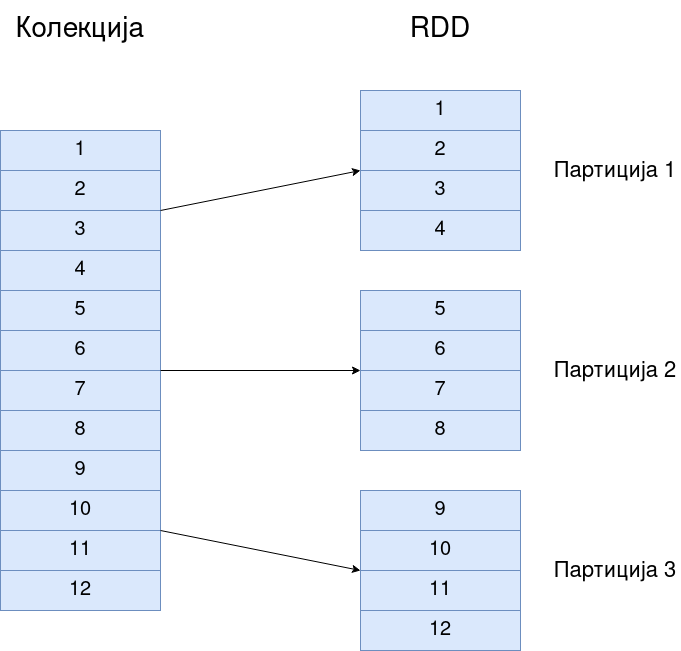
\includegraphics[width=0.80\textwidth]{pictures/spark_rdd_creation.png}
  \caption{Креирање \textit{RDD}-ja од колекције података}
  \label{fig:spark_rdd_creation_png}
\end{figure}

Данас се \textit{RDD} апстракција сматра застарелом и не користи се директно, већ постоје друге које су конструисане над њом и које су је потиснуле, углавном због бољих перформанси, попут \textit{Spark DataFrame}-a (поглавље \ref{sec:spark_df}).

\subsection{Трансформације}
\label{subsec:spark_transf}

\textit{Spark} је конструисан по принципима функционалног програмирања, па су све његове структуре података имутабилне, што значи да се након њиховог креирања не могу мењати \cite{spark_guide}. Пошто се подаци не могу мењати, свака операција која треба да их измени заправо креира потпуно нову струкуру података. На пример, уколико постоји \textit{RDD} којем се мењају подаци које садржи, они се неће изменити директно, већ ће се од постојећег \textit{RDD}-ја направити нови који у себи саржи измењене податке.

Тај процес, где се од једног \textit{RDD}-ја применом наредби добија други, се назива трансформација (енг. \textit{transformation})  \cite{spark_guide}. Пратећи функционалне концепте, трансформације немају бочне ефекте, што значи да се од једног \textit{RDD}-ја применом истих трансформација, као резултат увек добија исти \textit{RDD}, независно од тога када се те трансформације примењују. \textit{RDD} који трансформацијом настаје од другог \textit{RDD}-ја се назива зависни \textit{RDD} (енг. \textit{dependency}).

Постоје две различите врсте трансформација, уске (енг. \textit{narrow}) и широке (енг. \textit{wide}) \cite{spark_guide}. За уске трансформације важи да једна партиција у почетном \textit{RDD}-ју доприноси настајању највише једне партиције у зависном \textit{RDD}-ју. Са друге стране, широке трансформације су такве где једна партиција почетног \textit{RDD}-ја учествује у конструисању више партиција зависног \textit{RDD}-ја, често свакој. Обе врсте трансформација су приказане на слици \ref{fig:sprk_trnsf}. Из приказане слике се за широку трансформацију може приметити да се подаци унутар једне партиције изворног \textit{RDD}-ја премештају у сваку партицију зависног \textit{RDD}-ја. Та појава се другачије назива мешање (енг. \textit{shuffle}).

\begin{figure}[!ht]
  \centering
  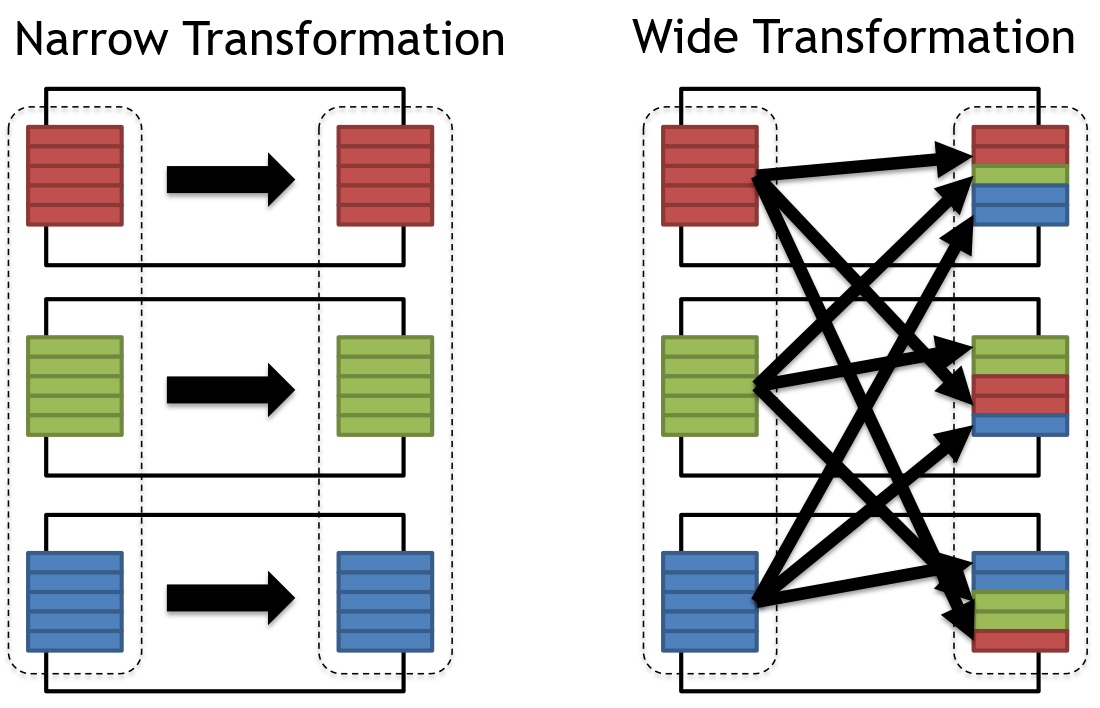
\includegraphics[width=1\textwidth]{pictures/spark_transformation_types.png}
  \caption{Приказ врста \textit{Spark} трансформација}
  \label{fig:sprk_trnsf}
\end{figure}

Постоји значајна разлика у перформансама узмеђу уских и широких трансформација \cite{spark_guide}. Код уских, \textit{Spark} извршава операције у меморији, док код широких пише резултате на диск и поново их распоређује по партицијама, што значајно успорава извршавање.

Све трансформације у \textit{Spark}-у припадају лењој евалуацији што значи да се не извршавају док се њихова вредности не затражи \cite{spark_guide}. За сваки ланац трансформација, \textit{Spark} креира \textit{план трансформација} који се извршава тек када је потребан њихов резултат. Евалуација скупа трансформација се у \textit{Spark}-у назива \textit{акција} (секција \ref{subsec:spark_akc}).

%\begin{comment} Разлог оваквог приступа је ефикасност. Уколико \textit{Spark} поседује информацију о томе које ће се све трансформације извршити над структуром података, може оптимизовати цео процес на такав начин да добијање резултата траје најкраће могуће. \end{comment}

%\subsubsection{Лења евалуација}
%\label{subsubsec:spark_lazy_eval}

%Лења евалуација је начин евалуације у коме се израз евалуира тек након што се његова вредност затражи. Све трансформације у \textit{Spark}-у припадају лењој евалуацији \cite{spark_guide}  . За сваки ланац трансформација, \textit{Spark} креира \textit{план трансформација} који се извршава тек када се ланац трансформација евалуира. Разлог оваквог приступа је ефикасност. Уколико \textit{Spark} има информацију о томе које ће се све трансформације извршити над неком структуром података, може оптимизовати цео процес на такав начин да добијање резултата траје најкраће могуће. Евалуација скупа трансформација у \textit{Spark}-у се назива \textit{акција} (секција \ref{subsec:spark_akc}).

\subsection{Примери \textit{RDD} трансформација}
\label{subsec:spark_transformation_types}

У \textit{Spark}-у постоји велики број трансформација, уских и широких. Неке од најпознатијих су приказане на слици \ref{fig:sprk_trnsf_examples} и то су:

\begin{description}
	\item[map,] за сваки елемент почетног скупа података производи нови, применом неке операције;
	\item[flatMap,] функционише исто као \textit{map} сa тим што сваки елемент почетног скупа произвноди нула, један или више елемената новог скупа;
	\item[filter,] од постојећег скупа елемената производи нови у коме се налазе они елементи почетног скупа који задовољавају некакав услов;
	\item[reduceByKey,] сабира вредности са заједничким кључем. Сабирање се иницијално извршава по партицији, након чега се подаци распоређују по новим партицијама и поново сабирају по кључу;
	\item[join,] спаја два скупа елемената у један, где ће резултат бити скуп података у коме је вредност сваког кључа унија вредности тог кључа у засебним скуповима који учествују у спајању.
\end{description}

\begin{figure}[!ht]
  \centering
  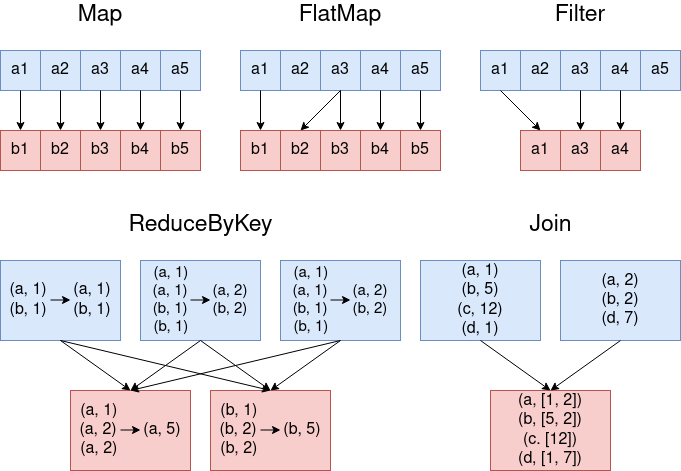
\includegraphics[width=1\textwidth]{pictures/transf_examples.png}
  \caption{Примери \textit{RDD} трансформација}
  \label{fig:sprk_trnsf_examples}
\end{figure}

Све \textit{RDD} трансформације су део \textit{Spark Core}-а \cite{spark_rdd_transf}. Поред поменутих, постоје и \textit{aggregate}, \textit{union}, \textit{intersect}, \textit{mapValues}, \textit{sortByKey} али и многе друге.


\subsection{Акције}
\label{subsec:spark_akc}

\textit{Spark} акције се користе када је потребно евалуирати резултат ланца трансформација \cite{spark_guide}. Уколико је резултат акције нека вредност, она се прослеђује драјвер програму. Постоје три врсте акција:

\begin{itemize}
\item акције које приказују резултат у конзоли;
\item акције које исписују резултат на излаз, на пример фајл;
\item акције које пребацују податке у колекцију програмског језика у коме се користи \textit{Spark}.
\end{itemize}

Као и трансформације, \textit{RDD} акције су део \textit{Spark Core}-а  \cite{spark_rdd_transf}. Неке од најкоришћенијих акција су:

\begin{description}
	\item[count,] исписује број елемената у структури података;
	\item[saveAsTextFile,] чува податке унутар \textit{RDD}-ја у текстуални фајл;
	\item[collect,] пребације све податке \textit{RDD}-ја у колекцију програмског језика;
	\item[take,] пребацује првих \textit{N} података \textit{RDD}-ја у колекцију програмског језика.
\end{description}

\subsection{Руковање грешкама}
\label{subsec:spark_dags}

У току извршавања \textit{Spark} трансформација могућа је појава грешака које могу да резултују губитком партиција. У том случају је \textit{Spark} у могућности да их поврати помоћу механизма који се назива граф наследства (енг. \textit{lineage graph}) у коме се чувају информације о томе од ког \textit{RDD}-ја је сваки \textit{RDD} у ланцу трансформација настао и применом којих трансформација. Пример једног ланца \textit{Spark} трансформација који у исто време представља и граф наследства је приказан на  слици \ref{fig:sprk_ppln}. Из примера се, на пример, може закључити да је \textit{RDD\_5} настао спајањем \textit{RDD\_2} и \textit{RDD\_4}.

\begin{figure}[!ht]
  \centering
  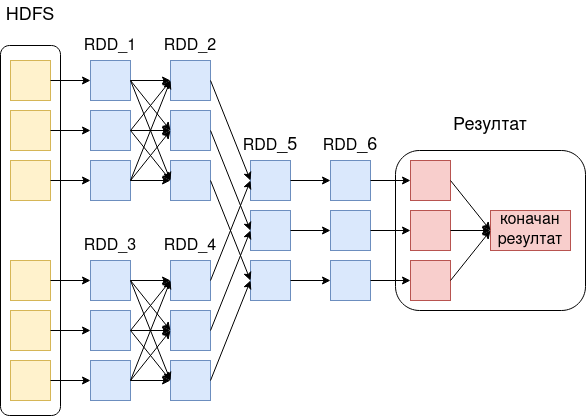
\includegraphics[width=0.9\textwidth]{pictures/spark_ppln.png}
  \caption{Пример једног \textit{Spark} извршавања}
  \label{fig:sprk_ppln}
\end{figure}

Уз помоћ графа наследства \textit{Spark} може да закључи од које партиције је настала свака партиција у ланцу и уколико нека од њих нестане, може је рекреирати \cite{hadoop_learning}. У случају да нека партиција ланца није исправна, \textit{Spark} ће проверити све партиције од којих је она настала. Уколико оне постоје, рекреираће неисправну партицију од њих, примењујући потребне трансформације. У супротном ће рекурзивно прегледати изворне партиције тих партиција и тај процес ће понављати све док се не пронађе исправна партиција или се не дође до партиције која је настала директним читањем са диска. У том случају ће је \textit{Spark} поново прочитати и након тога покренути ланац трансформација из почетка.

Процес рекреације партиција је поуздан из два разлога. Први је што трансформације немају бочне ефекте, па ће се рекреирањем увек добити исти \textit{RDD}. Други је што се изворни подаци чувају у \textit{HDFS}-у, који је поуздан, па ће се у случају поновног читања из меморије и рекреирања читавог ланца, увек прочитати почетна, непромењена, вредност са диска.

\subsection{Кеширање}
\label{subsec:spark_persist}

Веома битна карактеристика \textit{Spark}-а је могућност чувања података у меморији, односно кеширање \cite{spark_rdd}. Када се \textit{RDD} кешира, свака машина у кластеру ће у својој меморији сачувати партиције које се на њој налазе и касније их користити у акцијама или трансформацијама у којима је тај \textit{RDD} потребан, без извршавања целог ланца трансформација из почетка. Овакав приступ знатно побољшава перформансе \textit{Spark} апликације. Чување у меморији се извршава тек након што \textit{RDD} учествује у некој акцији. Кеширање је отпорно на грешке, и за рекреацију несталих партиција кешираног \textit{RDD}-ја се користи граф наследства.

\textit{RDD} се може кеширати коришћењем функција \textit{cache} и \textit{persist} \cite{spark_rdd}. Оне омогућавају различите нивое кеширања у зависности од тога у којој врсти меморије се партиције чувају:

\begin{description}
	\item[\textit{cache},] кешира податке у меморији;

	\item[\textit{persist},] са \textit{MEMORY\_ONLY} аргументом кешира податке у меморији;

	\item[\textit{persist},] са \textit{DISC\_ONLY} аргументом кешира податке на диску. Овај приступ се не саветује из тог разлога што је често брже рекреирати цео ланац трансформација из почетка, него учитати кеширан \textit{RDD} са диска;

	\item[\textit{persist},] са \textit{MEMORY\_ONLY\_2} аргументом кешира податке у меморији али поред тога извршава репликацију \textit{RDD}-ја на још једну машину кластера;

	\item[\textit{persist},] са \textit{DISC\_ONLY\_2} аргументом кешира податке на диску али поред тога извршава репликацију \textit{RDD}-ја на још једну машину кластера;

	\item[\textit{persist},] са {MEMORY\_AND\_DISC} аргументом кешира податке у меморији уколико постоји довољно простора, а у супротном кеширање извршава на диску.
\end{description}

\section{Апстракција података \textit{DataFrame}}
\label{sec:spark_df}

\textit{DataFrame} је дистрибуирана колекција налик табели, са дефинисаним редовима и колонама \cite{spark_guide}. Свака колона мора имати исти број редова и сваки ред мора имати исти број колона. Поред тога, свакој колони је додељен један тип ког морају бити све вредности које се у њој налазе.
% иако  можемо користити недостајуће вредности за број колона у редовима

Сваки \textit{Spark DataFrame} садржи метаподатке који описују имена колона и њихове типове  \cite{spark_guide}. Ти метаподаци се називају шема (енг. \textit{schema}). Шема се може дефинисати експлицитно али се може и аутоматски закључити из података који се налазе унутар \textit{DataFrame}-а. Поред типова, у шеми се налази информација о томе да ли колона може поседовати \textit{null} вредности. На слици \ref{fig:sprk_df_schema_example} је приказан једноставан пример \textit{DataFrame}-а и његове шеме.

\begin{figure}[!ht]
  \centering
  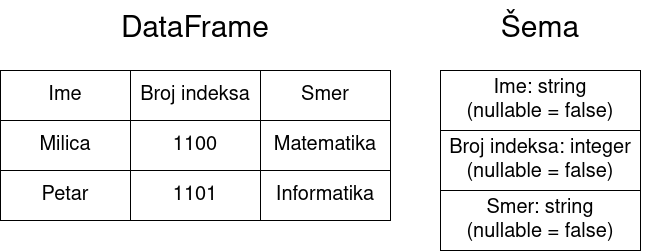
\includegraphics[width=1\textwidth]{pictures/dataframe_schema.png}
  \caption{\textit{Spark DataFrame} и његова шема}
  \label{fig:sprk_df_schema_example}
\end{figure}

У \textit{Spark}-у постоји велики број типова који се могу доделити колонама \textit{DataFrame}-а \cite{spark_guide}. Постоје једноставни типови попут целобројних бројева, децималних бројева и ниски али постоје и сложени, попут низова, мапа и датума. Сви \textit{Spark} типови се могу мапирати у одговарајуће типове програмских језика у којима се он користи.

\subsection{Трансформације и акције \textit{DataFrame}-а}
\label{subsec:spark_sql_ac_tr}

Све особине трансформација и акција које важе за апстракцију \textit{RDD}, важе и за трансформације и акције \textit{DataFrame}-а \cite{spark_guide}. Дакле, трансформације немају бочне ефекте и лењо се евалуирају, тек када се позове акција. Такође, резултат трансформације примењене на \textit{DataFrame} ће увек бити нови \textit{DataFrame}. Једина разлика је у томе што \textit{RDD} и \textit{DataFrame} другачије представљају податке, па су им трансформације и акције другачије. Како је \textit{DataFrame} сличан табели у релационим базама, поседује неколико трансформација које су идентичне наредбама у програмском језику \textit{SQL}. Неке од најкоришћенијх \textit{DataFrame} трансформација су приказане на слици \ref{fig:sprk_df_trnsf_example} и то су:

\begin{description} 
	\item[\textit{select},] конструише нови \textit{DataFrame} са подскупом колона почетног;
	\item[\textit{filter},] конструише нови \textit{DataFrame} са редовима почетног који задовољавају задати услов;
	\item[\textit{withColumn},] конструише нови \textit{DataFrame} додавањем колоне на почетни;
		\item[\textit{join},] спаја два \textit{DataFrame}-а у један на основу заједничких вредности колона.
\end{description}

\begin{figure}[!ht]
  \centering
  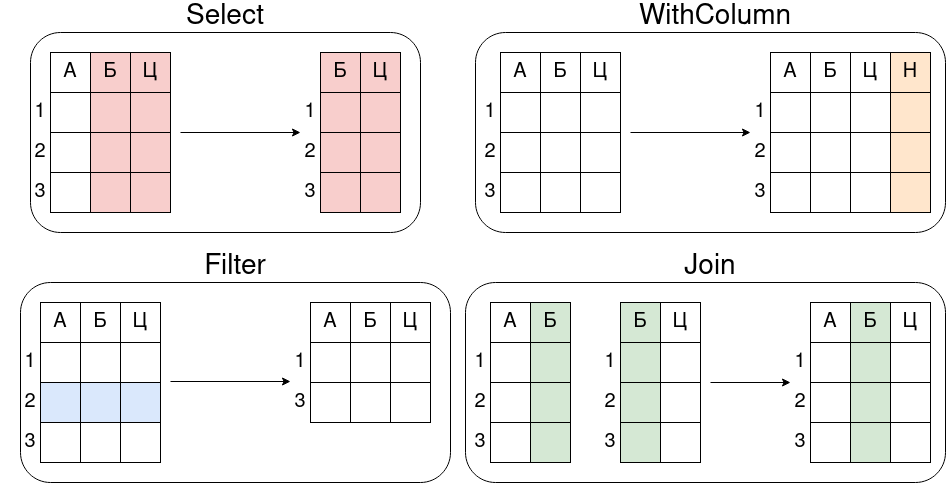
\includegraphics[width=1\textwidth]{pictures/df_trnsf_example.png}
  \caption{Примери \textit{DataFrame} трансформација}
  \label{fig:sprk_df_trnsf_example}
\end{figure}

Примери акција \textit{DataFrame}-а су \textit{collect}, која трансформише \textit{DataFrame} у струкуру података програмског језика у коме се \textit{Spark} користи и \textit{show}, која се користи за испис \textit{DataFrame}-а на стандардни излаз \cite{spark_guide}. Поред њих постоје и многе друге.

\subsection{Разлика између \textit{DataFrame}-а и \textit{RDD}-ја}
\label{subsec:spark_df_vs_rdd}

Поред различитог начина представљања података, постоји знатна разлика у перформансама између \textit{RDD}-ја и \textit{DataFrame}-а \cite{spark_guide}. \textit{RDD} се користи за програмирање ниског нивоа, пошто омогућава директан рад са партицијама. Међутим, приликом писања \textit{RDD} трансформација, програмер мора бити веома пажљив када и коју трансформацију примењује, због тога што редослед може значајно да утиче на перформансе.

Са друге стране, редослед примене трансформација \textit{DataFrame}-а не утиче на брзину извршавања \cite{spark_guide}. Разлог томе је што сваки \textit{DataFrame} к\^{о}д пролази кроз аутоматски процес оптимизације, па ће добијени резултат увек бити најбржи могући. За оптимизацију је задужен процес који се зове \textit{Catalyst}. Због перформанси, али и због једноставнијег интерфејса, \textit{DataFrame} је скоро потпуно потиснуо \textit{RDD} из употребе.

\subsection{Планови извршавања \textit{DataFrame}-а}
\label{subsec:spark_exec_plans}

%Процес извршавања \textit{DataFrame}-a се састоји из следећих корака:
%\begin{enumerate}
%\item К\^{o}д \textit{DataFrame}-а је написан
%\item уколико је исправан, од њега се прави логички план
%\item Од логичког плана се конструише физички план, уз примену оптимизација
%\item Добијени физички план се пребацује у \textit{RDD} и извршава се
%\end{enumerate}

Сваки \textit{DataFrame} се приликом покретања прво преводи у \textit{RDD}, након чека се извршава. Добијени \textit{RDD} к\^{о}д ће увек имати оптимизован редослед примена трансформација. Да би се оптимизација успешно изршила, \textit{Spark} током превођења генерише неколико планова извршавања.

Први план који се конструише од \textit{DataFrame} кода је неразрешен логички план (енг. \textit{unresolved logical plan}). Он представља трансформације које треба извршити над \textit{DataFrame}-ом, али не садржи никакве информације о томе над којим колононама, као ни о томе где се подаци које \textit{DataFrame} представља физички налазе \cite{spark_guide}. Те информације се добијају уз помоћ каталога (енг. \textit{catalog}) у коме се налазе информације о \textit{DataFrame}-овима. Резултат примене каталога на неразрешен логички план је логички план (енг. \textit{logical plan}). Анализом логичког плана и применом правила оптимизације на њега, оптимизатор \textit{Catalyst} конструише оптимизован логички план (енг. \textit{optimized logical plan}).

%Једно од правила \textbf{КАТАЛИСТА} се зове \textit{filter pushdown}. Његова улога је да \textit{filter} трансформације узврши што је раније могуће. На пример, у случају да \textit{DataFrame} чита податке из базе и након тога примењује \textit{filter}, долази до читања непотребих података. 

%\begin{figure}[!ht]
%  \centering
%  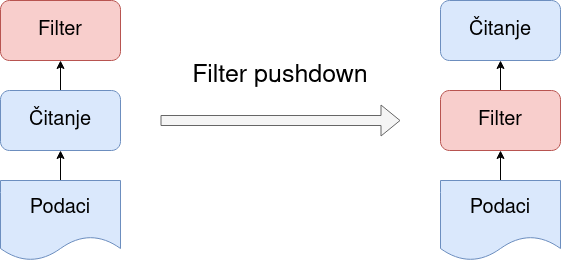
\includegraphics[width=1\textwidth]{pictures/filter_pushdown.png}
%  \caption{\textit{Filter pushdown}}
%  \label{fig:sprk_ex_plns}
%\end{figure}

Након што се оптимизовани логички план успешно креира, \textit{Spark} у односу на њега конструише неколико физичких планова (енг. \textit{physical plan}) \cite{spark_guide}. Физички план дефинише на који начин и уз помоћ којих наредби ће се логички план извршити на кластеру. Сви физички планови се након тога евалуирају и бира се онај са најбољим перформансама. Он се преводи у \textit{RDD} трансформације и ивршава на кластеру. Цео процес је приказан на слици \ref{fig:sprk_ex_plns}.

\begin{figure}[!ht]
  \centering
  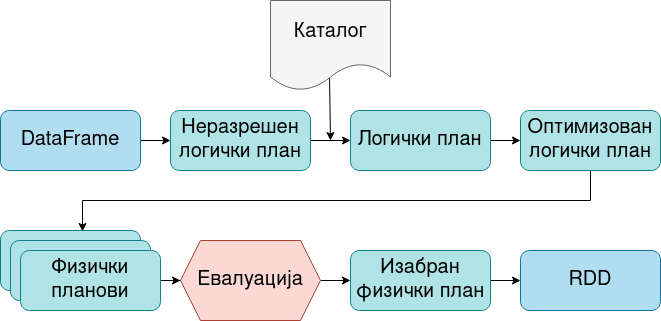
\includegraphics[width=0.85\textwidth]{pictures/dataframe_optimization.png}
  \caption{Ток извршавања \textit{Spark DataFrame}-a}
  \label{fig:sprk_ex_plns}
\end{figure}

\section{Остале компоненте \textit{Spark}-а}
\label{sec:spark_components}

\textit{Spark} омогућава коришћење \textit{SQL} упита над подацима. Сваки \textit{Spark SQL} упит пролази кроз исти процес оптимизације као и \textit{DataFrame} \cite{spark_guide}. Једина разлика је у томе што се синтаксне грешке \textit{SQL} кода појављују током извршавања програма, док се синтаксне грешке \textit{DataFrame} кода појављују приликом компилације. У коду \ref{lst:sprk_sql_df_slct_example} је приказано када долази до појаве грешке приликом покретања еквивалентних \textit{DataFrame} и \textit{SQL} наредби са погрешно написаном речи \textit{select}.  

\begin{lstlisting}[language=Python, caption={Извршавање \textit{DataFrame} и  \textit{SQL} кодова са грешком у писању}, label={lst:sprk_sql_df_slct_example}]
# Spark DataFrame
dataframe.slect()
>>> compilation error

# Spark SQL
spark.sql('slect * from dataframe')
>>> runtime error
\end{lstlisting}

Поред апстракција података \textit{RDD} и \textit{DataFrame}, постоји и \textit{DataSet}, који је доступан само у \textit{JVM} базираним језицима, Скали и Јави \cite{spark_guide}. Представља податке на исти начин као \textit{DataFrame} и пролази кроз исти процес оптимизације. Разлика је у провери типова вредности унутар колона, која се код \textit{DataFrame}-а дешава током извршавања програма, док се код \textit{DataSet}-а извршава за време компилације.

Уз помоћ \textit{Spark}-а се могу конструисати модели машинског учења, преко \textit{Spark MLlib} библиотеке \cite{spark_guide}. Она се може користити за препроцесирање, тренирање модела и прављење предвиђања. \textit{Spark} поседује и библиотеку за рад са графовима, \textit{GraphX}, али се због њених разних недостатака, за обраду графова на кластеру често користе друга решења.

\textit{Spark} се може користити и за операције над токовима података \cite{spark_streaming}. \textit{Spark streaming} омогућава претплату на токове који настају из веб сокета (енг. \textit{web socket}), локације у фајл систему или од стране \textit{Apache Kafka}-е. Након претплате, на податке у току се могу примењивати исте трансформације као код \textit{DataFrame}-а.

% ако хоћеш да причаш о каталисту можеш наћи овде https://databricks.com/blog/2015/04/13/deep-dive-into-spark-sqls-catalyst-optimizer.html

% -------------------------------------
\begin{comment} % -------------------------------------
% -------------------------------------

\chapter{Семантички веб}
\label{chp:sem_veb}

Веб је током свог постојања константно еволуирао. Разликују се три веће етапе које су назване по редним бројевима, Веб 1.0, Веб 2.0 и Веб 3.0.

\section{Веб 1.0}
\label{sec:sem_veb_veb_1}

Ова верзија представља прву фазу еволуције веба. Настао је у последњим деценијама 20. века и трајао је до средине прве деценије 21. Карактерише га скуп статичког садржаја који је повезан преко веза названих \textit{hyperlik}.

Уз помоћ њега су представљане само информације које су се приказивале корисницима. Још увек није постојао језик за улепшавање страница, \textit{CSS} и није било динамичких линкова, логовања корисника и остављања коментара.

%Веб страница Свемирског баскета (енг. \textit{Space Jam}), популарног филма из 90-тих нам даје увид у то како је изгледала једна страница тада, пошто је непромењена од тренутка када је направљена, 1996. године. Можемо је пронаћи на адреси https://www.spacejam.com/1996/.

%\begin{figure}[!ht]
%  \centering
%  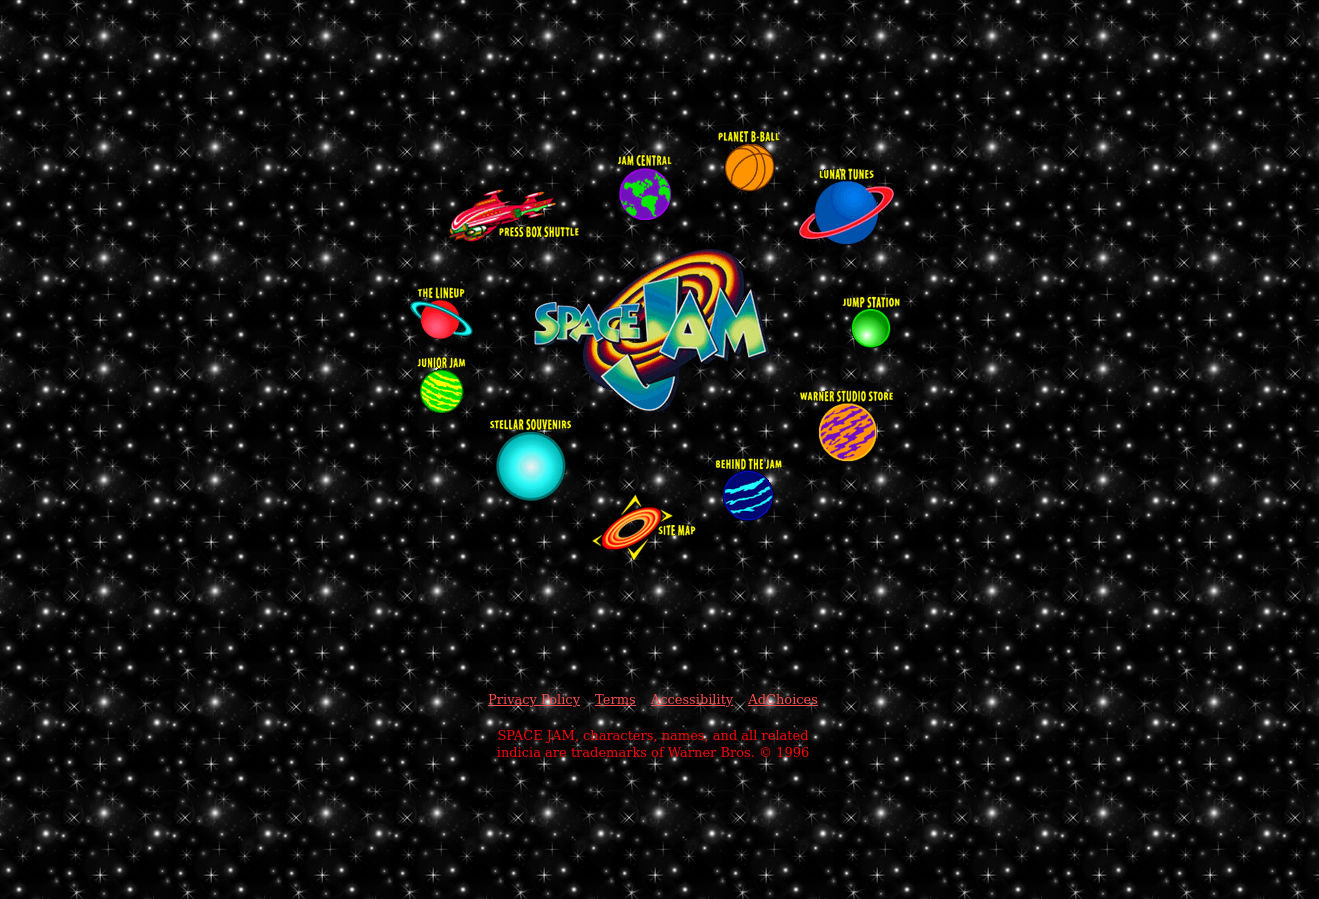
\includegraphics[width=1\textwidth]{pictures/space_jam.png}
%  \caption{Веб страница Свемирског баскета}
%  \label{fig:sem_veb_space_jam}
%\end{figure}

\section{Веб 2.0}
\label{sec:sem_veb_veb_2}

Друга фаза је почела одмах након прве и траје и дан данас. Акценат је стављен на садржај генерисан од стране корисника, једноставно коришћење као и на размени информација. У овој фази је, преко програмских језика који се извршавају на серверској страни, омогућен рад разних апликација попут Амазона (енг. \textit{Amazon}), Ју Тјуба (енг. \textit{YouTube}) и Фејсбука (енг. \textit{Facebook}). Све то је омогућило корисницима да на једноставан начин деле и размењују своја мишљења и искуства.

%\begin{figure}[!ht]
%  \centering
%  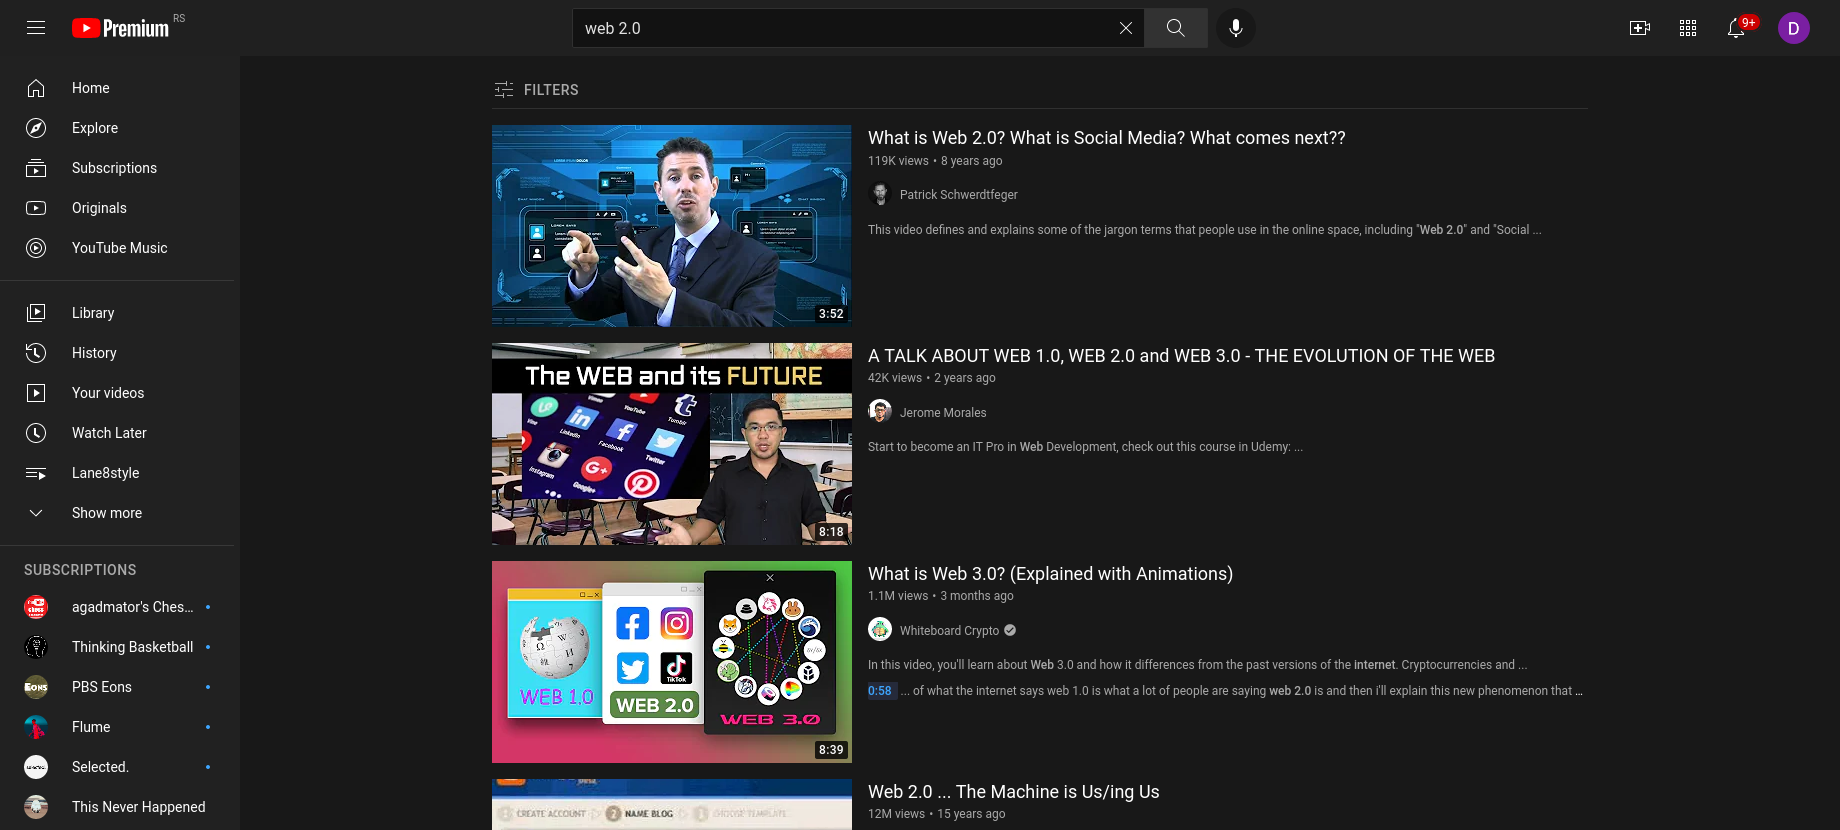
\includegraphics[width=1\textwidth]{pictures/youtube_page.png}
%  \caption{YouTube веб страница}
%  \label{fig:sem_veb_you_tube_page}
%\end{figure}

Међутим, Веб 2.0 има једну велику ману, а то је да се сви подаци, које поменуте апликације сакупљају, складиште на приватним серверима које контролишу корпорације. Велики број њих користи те податке да би кориснике што дуже задржалo на својим сервисима. Такође, у неколико инстанци су ти подаци продавани некој другој страни, у циљу једноставне зараде. Због овога се може рећи да су корисници постали производ друге фазе веба.

\section{Веб 3.0}
\label{sec:sem_veb_veb_3}

Циљ треће верзије веба је да се ослободи централизације присутне у вебу 2.0 и направи децентрализован али сигуран интернет где би људи могли да размењују информације без посредника, ког тренутно представља корпорација чије услуге ти корисници користе.

Последица децентрализације је та да апликације више неће бити покретане преко огромних, приватних, база података и сервера, већ ће се прећи на технологије као што су блокчеин (енг. \textit{blockchain}) и мреже равноправних корисника (енг. \textit{peer-to-peer}).

Идеја је да у самом срцу веба 3.0 стоји семантички веб, чија би улога била да повеже постојеће податке и информације које се налазе на интернету, и направи их таквим да њихов садржај и контекст могу разумети машине.

\begin{figure}[!ht]
  \centering
  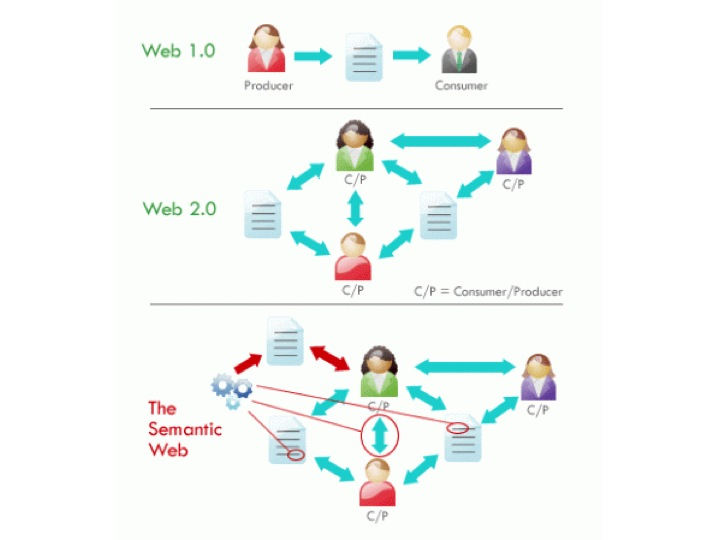
\includegraphics[width=1\textwidth]{pictures/webs_vrs.jpg}
  \caption{Фазе Веба}
  \label{fig:sem_veb_versions}
\end{figure}

Ова верзија Веба је још увек у развоју, са огромним простором за даље истраживање. Међутим, како је сама архитектура доста комплекснија од архитектуре Веба 2.0, није сигурно да ли ће заживети и ако да, када. Али оно што је сигурно је да идеја о дељеним подацима и децентализованом вебу и даље постоји и велики број људи је развија и унапређује.

%Један од примера веб 3.0 апликације је \textit{odysee} направљена за дељење видео снимака и сматра се децентрализованом алтернативом \textit{YouTube}-a. Ова апликација користи \textit{LBRY} протокол \cite{lbry} који је базиран на блокчеин технологији и користи се за дељење фајлова и плаћање. \cite{odysee_article}

%Тим који стоји иза ове апликације сматра да је \textit{YouTube} превише стриктан у томе који садржај бира да промовише и блокира. \textit{Odysee} je настала са идејом слободе говора и направљена је тако да је свако може користити да промовише своје погледе на свет. \cite{odysee_article}

%Идеја иза веба 3.0 је таква да интернет више не контролишу компаније које поседију сервере, већ да се та контрола пребаци на кориснике. Самим тим, информације о корисницима се више неће налазити на приватним серверима, већ ће бити пребачене код самих корисника, уз помоћ блокчеин технологије.  \cite{coinbase_web3}

%То доводи до огрмоних промена у томе како веб функционише. Архитектура веба 2.0 је једноставна. Састоји се од клијента, који је обично представљен интернет претраживачем или неком апликацијом, који комуницирају са серверима и од њих добијају информације уз помоћ којих функционишу. Ентитет који контролише сервере, контролише и који корисници могу да им приступају као и шта они могу да виде, па стога, један корисник може имати привилегован статус у односу на другог. Поред тога, чува информације о поменутим корисницима и о томе шта они на тим серверима поседују. \cite{coinbase_web3}

%У вебу 3.0, апликацијама је дозвољено да чувају садржај на јавно доступном блокчеину. Дакле, тај садржај постаје доступан свима. Такође, дозвољава корисницима директну контролу над тим садржајем. Идеја је да не постоји потреба за корисничким налозима или привилегованим АПИ (енг. \textit{API}) кључевима, већ да свако може да приступи свему. 

%Веб 3.0 то омогућава уз помоћ употребе крипто новчаника (енг. \textit{crypto wallet}), уз помоћ ког наша апликација шаље трансакције на блокчеин, и блокчеин чворова (енг. \textit{blockchain node}), чија је улога да надгледају и регистрију трансакције које се дешавају на блокчеину. \cite{coinbase_web3}

%Када крипто новчаник жели да пошаље неку трансакцију на блокчеин или када од њега захтева некакве информације, комуницираће са блокчеин чворовима. Преко тога је нашој апликацији омогућено да комунуцира са блокчеином и на тај начин она сакупља информације које су јој потребне да би правилно функционисала. Овај однос подсећа на однос који данашње апликације имају са својим приватним серверима. \cite{coinbase_web3}

%Поређење архитекура између две верзије веба је приказано на слици \ref{fig:sem_veb_veb3_arh}.

% https://www.coinbase.com/learn/crypto-basics/what-is-a-crypto-wallet

%\begin{figure}[!ht]
%  \centering
%  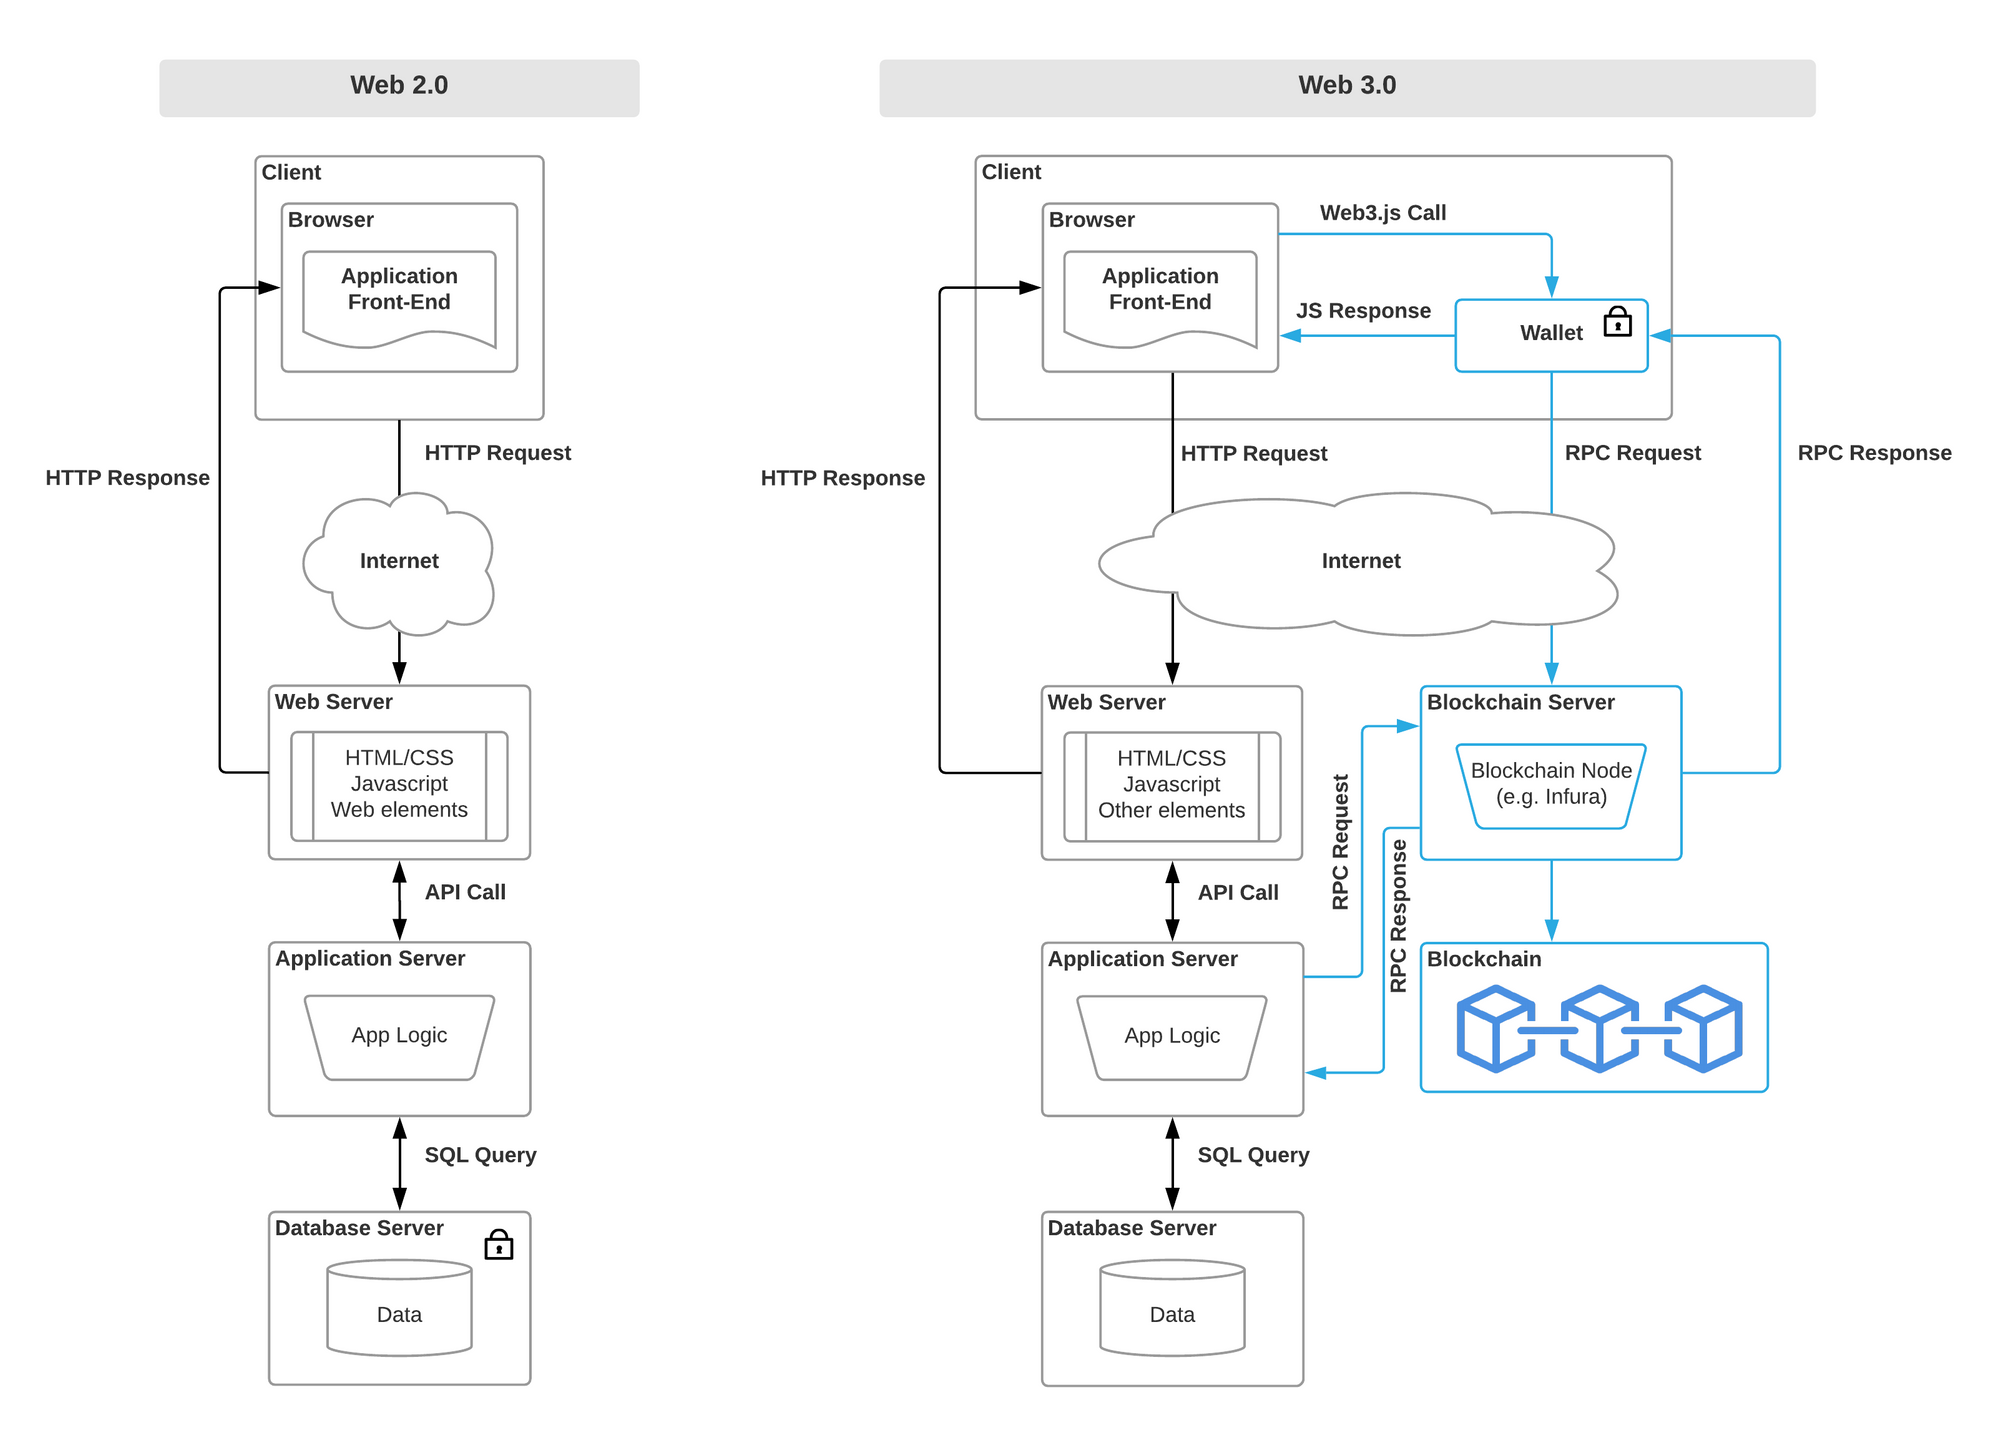
\includegraphics[width=1\textwidth]{pictures/veb3_arh.png}
%  \caption{Једноставан приказ архитектура веба 2.0 и веба 3.0}
%  \label{fig:sem_veb_veb3_arh}
%\end{figure}

%Наравно, веб 3.0 доноси и неколико проблема. Прво, тренутне машине које се користе за рударење криптовалута и праћење трансакција конзумирају огромне количине енергије, па ће стога њена потрошња бити велики проблем који се мора решити пре него што веб 3.0 постане стварност.

%Такође, сви подаци ће се и даље налазити на серверима али ти сервери неће бити у приватном власништву великих корпорација. То доноси неколико питања. На пример, ко је власник тих сервера? Ко плаћа нихово одржавање? Ко има информације о нашим налозима, попут шифри које користимо и других личних података? Дакле, неко ће ипак бити власник наших података, с тим што се поставља питање, ко тачно?

% https://www.stephendiehl.com/blog/web3-bullshit.html

%Ова верзија веба је још увек нова, са огромним простором за даље истраживање али се због свега наведеног није сигурно да ли ће икада заживети, и ако да, када? Оно што је сигурно да идеја о дељеним подацима и децентализованом вебу и даље постоји и велики број људи је развија и унапређује. У самом средишту дељења података се налази семантички веб.

\section{Семантички веб}
\label{sec:semantic_veb_main}

Семантички веб је надоградња садашњег веба, \textit{WWW}-а, који омогућава рачунарима да, на интелигентан начин, претражују и обрађују податке са веба. Интелигентно у овом случају значи да ће рачунари бити способни да закључе шта подаци представљају људима који их користе. Пошто до сада није конструисан ниједан систем вештачке интелигенције који може потпуно да опонаша човека, то се може постићи само ако се значење, то јест семантика, ресурса на вебу експлицитно представи рачунарима у формату у којем их они могу обрадити. \cite{semantic}

Да би се ово постигло, није довољно само складиштити податке у језику који машине разумеју, на пример у \textit{HTML} формату, већ је неопходно да се уз те податке додају и информације о семантици која јасно говори које закључке треба из њих извући. Међутим, тако нешто је врло вероватно немогуће извести због тога што је чак и људима тешко да се договоре око значења садржаја одређених страница на вебу, па је стога још теже формализовати тај садржај на такав начин да буде значајан машинама. \cite{semantic}

%Дакле, семантички веб заправо има намену да омогући машинама приступ већем броју информација, којима је до сада приступао само човек, у на тај начин доведе до смањења потрошње времена корисника интернета.
%То значи да семантички веб заправо има другу намену, а то је омогући машинама приступ  већем броју информација којима тренутно приступа човек, што доводи до смањења потрошње времена. То значи да семантички веб заправо није екстензија данашњег веба, већ некакав идеал ка коме веб временом еволуира. \cite{semantic}

Да би семантички веб функционисао, на неки начин се људско знање мора изразити неким формалним језиком. Тај проблем се може решити моделовањем. Један од језика који се користи у семантичком вебу је \textit{OWL 2} и настао је под утицајем коришћења моделовања у биологији. На који начин ће знање бити моделовано зависи од тога за шта ће конструисан модел бити коришћен. Код семантичког веба, идеја је да компјутерски програми закључују на основу датих информација на такав начин да узимају у обзир резоновање и формалну репрезентацију знања. \cite{semantic}

Дакле, развој семантичког веба се заснива на припајању моделовања знања и аутоматског закључивања вебу. Исто тако, на овај начин се веб апликације уводе у домен формалног моделовања и репрезентације знања. 

Иако су раније постојали примери стандардизације саме формалне репрезентације знања, семантички веб је допринео њеној важности и употребљивости. Велика већина релевантних покушаја стандардизације је спроведена од стране \textit{WWW} Конзорцијума, познатијег као \textit{W3C}. \cite{semantic}

%Исто тако, сам Веб у друге дисциплине уводи појам дистрибуираних али повезаних информација. Веб ставља акценат на важност јасно дефинисаних, стандардизованих језика који се користе за размену података између различитих јединица. 

\subsubsection{Историјат}
\label{subsubsec:semantic_timeline}

Идеја додељивања семантике вебу није нова и постојала је још у самом зачећу веба. Први покушаји су забележени код типизираних линкова (енг. \textit{typed links}) чија је улога била да, поред тога што су представљали референцу ка другом документу, садрже и неке информације о томе шта заправо тај линк представља. \cite{semantic}

Семантички веб је добио већу пажњу јавности 2001. године, када је Тим Бернерс Ли (енг. \textit{Tim Berners-Lee}) објавио чланак назван \textit{Семантички веб} у којем су представљене идеје о томе како би семантички веб функционисао. До данас је \textit{W3C}, чији је Тим Бернерс Ли члан, објавио неколико технологија међу којима су \textit{RDF, Resоurce Description Framework}, \textit{OWL, Web Ontology Language} и језик за упите \textit{SPARKQL}, али и многе друге. \cite{semantic}

Поред тога су забележени и покушаји у томе да се у \textit{HTML} документе, преко вредности атрибута, доделе неки семантички подаци једном веб документу. Те вредности се називају микроформати (енг. \textit{microformats}) и користе се за решавање проблема у специфичним доменима апликација, на пример, приликом енкодирања личних података. \cite{semantic}

Једноставан пример микроформата је \textit{HTML} атрибут \textit{rel} који се користи да би се назначило шта се налази на линку коме тај атрибут је додељен. У следећем примеру се користи да би се нагласило да се на приложеном линку налази лиценца.

\begin{lstlisting}[language=HTML]
<small>This article is licensed under a 
  <a rel="license" href="http://creativecommons.org/licenses/by-nc-sa/2.0/">
  Creative Commons Attribution Non-commercial Share-alike 
  (By-<abbr>NC</abbr>-<abbr>SA</abbr>) license</a>.
</small>
\end{lstlisting}

Количина семантичких података која је доступна на вебу се повећава из године у годину и подаци су постали међусобно повезани. Ово се дешава због тога што идентификатори који се користе у језицима семантичког веба прате исте принципе као и адресе класичног веба. Стога, име једног објекта семантичког веба се може интерпретирати као веб адреса. То доводи до појаве повезаних података (енг. \textit{linked data}) која се односи на семантичке податке чији су идентификатори заправо показивачи ка веб адресама на којима се може пронаћи више информација о објекту. \cite{semantic}

Због тога се користи термин \textit{веб података}, који описује семантички веб као покушај који се примарно фокусира на размену података. 

\subsection{RDF језик}
\label{subsec:semantic_rdf}

Механизам за описивање ресурса (енг. \textit{resource description framework}) или скраћено \textit{RDF} је формални језик за описивање структуираних информација. Поента овог језика је да омогући апликацијама да размењују податке на вебу задржавајући њихово оригинално значење. За разлику од језика као што су \textit{HTML} и \textit{XML}, циљ није приказати документе у правилном формату већ омогућити обраду информација које они садрже. Због свега наведеног \textit{RDF} се често сматра основом за развој семантичког веба. \cite{semantic}

Дакле, улога \textit{RDF}-а није да описује структуру докумената, већ да опише однос између неких објеката. Данас је овај формат веома распростањен и готово сваки виши програмски језик поседује библиотеке помоћу којих се могу извршавати разне операције над њим. \cite{semantic}
 
\textit{RDF} документ је описан усмереним графом, односно скупом чворова који су повезани усмереним гранама. Сваки чвор и свака грана имају засебан идентификатор. Структура графа је изабрана баш из тог разлога да би се изразио однос између објеката, а не њихова хијерархија. На пример, на слици \ref{fig:semantic_rdf_graph_example} се примећује да је однос између приказаних елемената, курса и студената, информација која нема јасну хијерахију. \textit{RDF} користи такав однос као основну јединицу информације. Штавише, велики број таквих односа производи графове. \cite{semantic}

\begin{figure}[!ht]
  \centering
  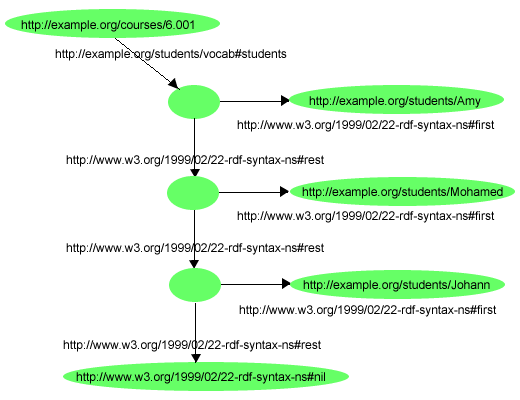
\includegraphics[width=0.8\textwidth]{pictures/rdf_graph_example.png}
  \caption{Пример РДФ графа}
  \label{fig:semantic_rdf_graph_example}
\end{figure}

Други разлог због кога је \textit{RDF} представљен графом је чињеница да му је улога да служи као описни језик података веба и других мрежа. Иформације у овим срединама се складиште и обрађују дистрибуирано па је стога битно комбиновати \textit{RDF} податке на једноставан начин. На пример, граф који је репрезентација једних података се лако може повезати са графом који представља нешто друго, једноставним повезивањем. Ако претпоставимо да поред графа на слици \ref{fig:semantic_rdf_graph_example} постоји, на пример, још један граф који описује студенте, лако се може закључити да се они једноставно могу повезати и користити заједно. \cite{semantic}

Додељивање имена \textit{RDF} документима може произвести проблеме. Наиме, именовање не мора бити униформно. На пример, могуће је да два документа садрже информације о истој теми, али да су им идентификатори потпуно различити. Такође, могуће је и да је једном истом ресурсу додељено неколико различитих имена или да се исти идентификатори користе за различите појмове.

Да би се тај проблем избегао \textit{RDF} користи униформни индикатор ресурса (енг. \textit{uniform resource identificator, URI}) као имена, у циљу разликовања ресурса. Напоменимо да је \textit{URI} генерализација \textit{URL} адреса које се користе за приступ документима на интернету. Како је сваки \textit{URL} валидан \textit{URI}, може се користити као идентификатор унутар \textit{RDF} докумената. У великом броју апликација циљ није разменити информације о веб страницама већ о великом броју објеката као што су на пример студенти, књиге, места, догађаји и тако даље. Таквим објектима се не може приступити на интернету па се њихов \textit{URI} користи ускључиво за идентификацију. Напоменимо и то да се \textit{URI} адресе које нису \textit{URL} називају \textit{URN}. \cite{semantic}

Због идентификације, чворовима и гранама унутар \textit{RDF} графа се додељује \textit{URI} као име, што можемо приметити и на већ приложеном примеру (слика \ref{fig:semantic_rdf_graph_example}). Ово правило има два изузетка. Први је тај да је ипак могуће доделити име које није \textit{URI}, а други је да је могуће не доделити име и оставити га празним, али се таквим случајевима нећемо бавити. \cite{semantic}

Иако \textit{URI} представљају имена, њихово значење је подложно интерпретацији па другачији алати могу на другачији начин да посматрају њихово значење. Због тога је уведен још један појам, литерал, који представља вредности унутар \textit{RDF}-а. Увек су записани ниском уз коју је припојен и њен тип. На пример, ниска \textit{"123"} може бити целобројног типа што би значило да представља број \textit{123}. За разлику од \textit{URI}-ја, литерали увек имају једно значење. У графу се представљају правоугаоним чворвима (слика \ref{fig:sem_rdf_graph_2})). \cite{semantic}

\begin{figure}[!ht]
  \centering
  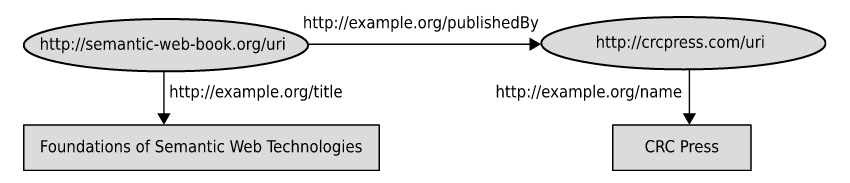
\includegraphics[width=0.8\textwidth]{pictures/rdf_graph_example_2.png}
  \caption{Пример РДФ графа са литералима}
  \label{fig:semantic_rdf_graph_2}
\end{figure}

\subsubsection{Репрезентација}
\label{subsubsec:semantic_rdf_representation}

Како су \textit{RDF} графови ретки, представљају се скупом грана које се у њему налазе. Једна грана је представљена вредношћу чворова, као и њеном ознаком. Чворове називамо субјекат и објекат, док се ознака назива предикатом. Тројка субјекат-предикат-објекат се другачије назива и \textit{RDF} тројком. Сваки члан тројке може бити некакав \textit{URI} али може бити и литерал. \cite{semantic}

Један од формата који се користе за репрезентовање \textit{RDF} графа је корњача (енг. \textit{turtle}) нотација. У овој нотацији се граф са слике \ref{fig:semantic_rdf_graph_2} приказује на следећи начин:

\begin{lstlisting}[language=XML]
<http://semantic-web-book.org/uri> <http://example.org/publishedBy> <http://crcpress.com/uri> .
	
<http://semantic-web-book.org/uri> <http://example.org/title> "Foundations of Semantic Web Technologies" .

<http://crcpress.com/uri> <http://example.org/name> "CRC Press" 
\end{lstlisting}

Међутим, овај запис, тачније \textit{URI} који му припадају, се може скратити увођењем префикса који означавају именска поља која представљају фамилију \textit{URI} адреса. Уз помоћ њих се исти запис може записати доста једноставније:

\begin{lstlisting}[language=XML]
@prefix book: <http://semantic-web-book.org/> .
@prefix ex: <http://example.org/> .
@prefix crc: <http://crcpress.com/> .

book:uri ex:publishedBy crc:uri .
book:uri ex:title "Foundations of Semantic Web Technologies" .
crc:uri ex:name "CRC Press" .
\end{lstlisting}

Поред корњача нотације, чест начин репрезентовања \textit{RDF} структуре је уз помоћ \textit{XML} формата. Разлог томе је што је тај формат читљив и људима и машинама, али и тај што скоро сваки програмиски језик поседује алате за обраду тог формата. Приказ једноставног \textit{RDF} графа са слике \ref{fig:semantic_rdf_graph_2} у \textit{XML} формату се може наћи у наставку:

\begin{lstlisting}[language=XML]
?xml version="1.0" encoding="utf-8"?>
<rdf:RDF xmlns:rdf="http://www.w3.org/1999/02/22-rdf-syntax-ns#"xmlns:ex ="http:/example.org/">
  <rdf:Description rdf:about="http://semantic-web-book.org/uri">
    <ex:publishedBy>
      <rdf:Description rdf:about="http://crcpress.com/uri">
      </rdf:Description>
    </ex:publishedBy>
  </rdf:Description>
</rdf:RDF>
\end{lstlisting}

%РДФ шема, страна 46 у књизи. можда то да додаш (\textit{RDF})

%\textbf{Chapter 7
%Query Languages
%In previous chapters, we learned about a number of possibilities for specifying
%information in a machine-readable way. RDF allows us to structure and relate
%pieces of information, and RDFS and OWL introduced further expressive
%means for describing more complex logical relations. The latter was further
%extended by means of logical rules that could be combined with OWL. For
%each of those description languages, we also introduced a notion of logical
%entailment: RDF(S) documents may entail other documents (Chapter 3),
%and OWL knowledge bases – possibly augmented with rules – can imply new
%axioms (Chapters 4, 5, 6)}


\subsection{OWL}
\label{subsec:semantic_owl}

\textit{OWL}, скраћено од \textit{Web Ontology Language}, је језик семантичког веба који се користи за представљање комплексног знања о стварима, њиховим групама или њиховим релацијама. Комплексно знање у овом контексту су инфомације које се не могу изразити преко \textit{RDF} формата. Овај језик спада у групу логичких језика, па се знање које изражава може користити унутар компјутерских програма. \textit{OWL} документ се назива онтологијом и могуће га је поставити на интернет, одакле га могу реферисати неке друге \textit{OWL} онтолигије. \cite{semantic}

Тренутна верзија овог језика је \textit{OWL 2}. 

%https://www.w3.org/2001/sw/wiki/OWL

\subsection{SPARQL}
\label{subsec:semantic_query}

Иако се информације из претходно поменутих \textit{RDF} и \textit{OWL} формата могу сазнати њиховом обрадом, то често у пракси није довољно. Због тога су настали упитни језици, чија је улога извлачење потребних информација из разних структура података семантичког веба. Упитни језик за \textit{RDF} је назван \textit{SPARKQL}. \cite{semantic}

Спаркл, или \textit{SPARQL}, \textit{SPARQL protocol and RDF query language}, је стандард за упите информација \textit{RDF} формата као и за представљање добијених резултата. Иако је синтакса овог језика веома слична синтакси језика \textit{SQL}, користе се за упите над тотално другачијим структурама података. \cite{semantic}

Пример једног \textit{SPARQL} упита је приказан у наставку.

\begin{lstlisting}[language=XML]
PREFIX ex: <http://example.org/>
SELECT ?title ?author
WHERE { 
	?book   ex:publishedBy   <http://crc-press.com/uri> .
	?book   ex:title         ?title .
	?book   ex:author        ?author 
}
\end{lstlisting}

Приказани упит се састоји из три дела. Први део је одређен са речи  \textit{PREFIX} и означава именски простор, исто као у корњача нотацији. Након њега следи \textit{SELECT} који одређује формат резултата који ће бити приказан. Трећа фаза, у којој се заправо упит и извршава, је означена са \textit{WHERE} коју прати некакав приказ графа. У приказаном примеру је граф представљен са три тројке које означавају која правила морају да важе за информације које упитом желимо да добијемо. У овом случају су то наслови и аутори чланака које је објавио \textit{CRC Press}, таквих да наслов и аутор постоје. \cite{semantic}

Наравно, Спаркл језик је доста мођнији од једноставног примера који је приказан, али улазак у детаље је ван опсега овог рада.

%query languages, chapter 7
%https://www.w3.org/2001/sw/wiki/SPARQL

\subsection{Употреба семантичког веба}
\label{subsec:semantic_end}

Семантички веб је и даље млада технологија која се развија, и тренутно се налази у фази између примене и развоја, али има велики потенцијал и може имати велики број примена. У последње време неке веб странице и портали почињу да користе \textit{RDF} и метаподатке и на тај начин постају део уланчаних података (енг. \textit{linked data}). У последње време се појављују и семантичке википедије, које су сличне као и већ постојеће, с тим што омогућавају кориснику да мења метаподатке који допуњује странице. Поред њих се развијају и семантички портали, веб странице где поред информација доступних човеку, постоје и друге, онтолошке, намењене машинама. Те информације се користе у циљу побољшања искуства корисника који користе те портале. \cite{semantic}

% https://www.w3.org/standards/semanticweb/
% http://people.mpi-inf.mpg.de/~dstepano/KRSW/literature/SWTechnologies.pdf

% -------------------------------------
\end{comment} % -------------------------------------
% -------------------------------------

\chapter{Скуп података \textit{OpenStreetMap}}
\label{chp:osm}

\textit{OpenStreetMap}, скраћено \textit{OSM}, је бесплатна мапа света која дозвољава приступ географским мапама, као и подацима које те мапе садрже \cite{osm_wiki}. Основна идеја овог пројекта је да заједница корисника развија и одржава мапе које представљају алтернативу већ постојећим мапама, попут оних које развија \textit{Google} \cite{google_maps}. Пример \textit{OSM} мапе на вебу је приказан на слици \ref{fig:osm_map_example}.

\begin{figure}[!ht]
  \centering
  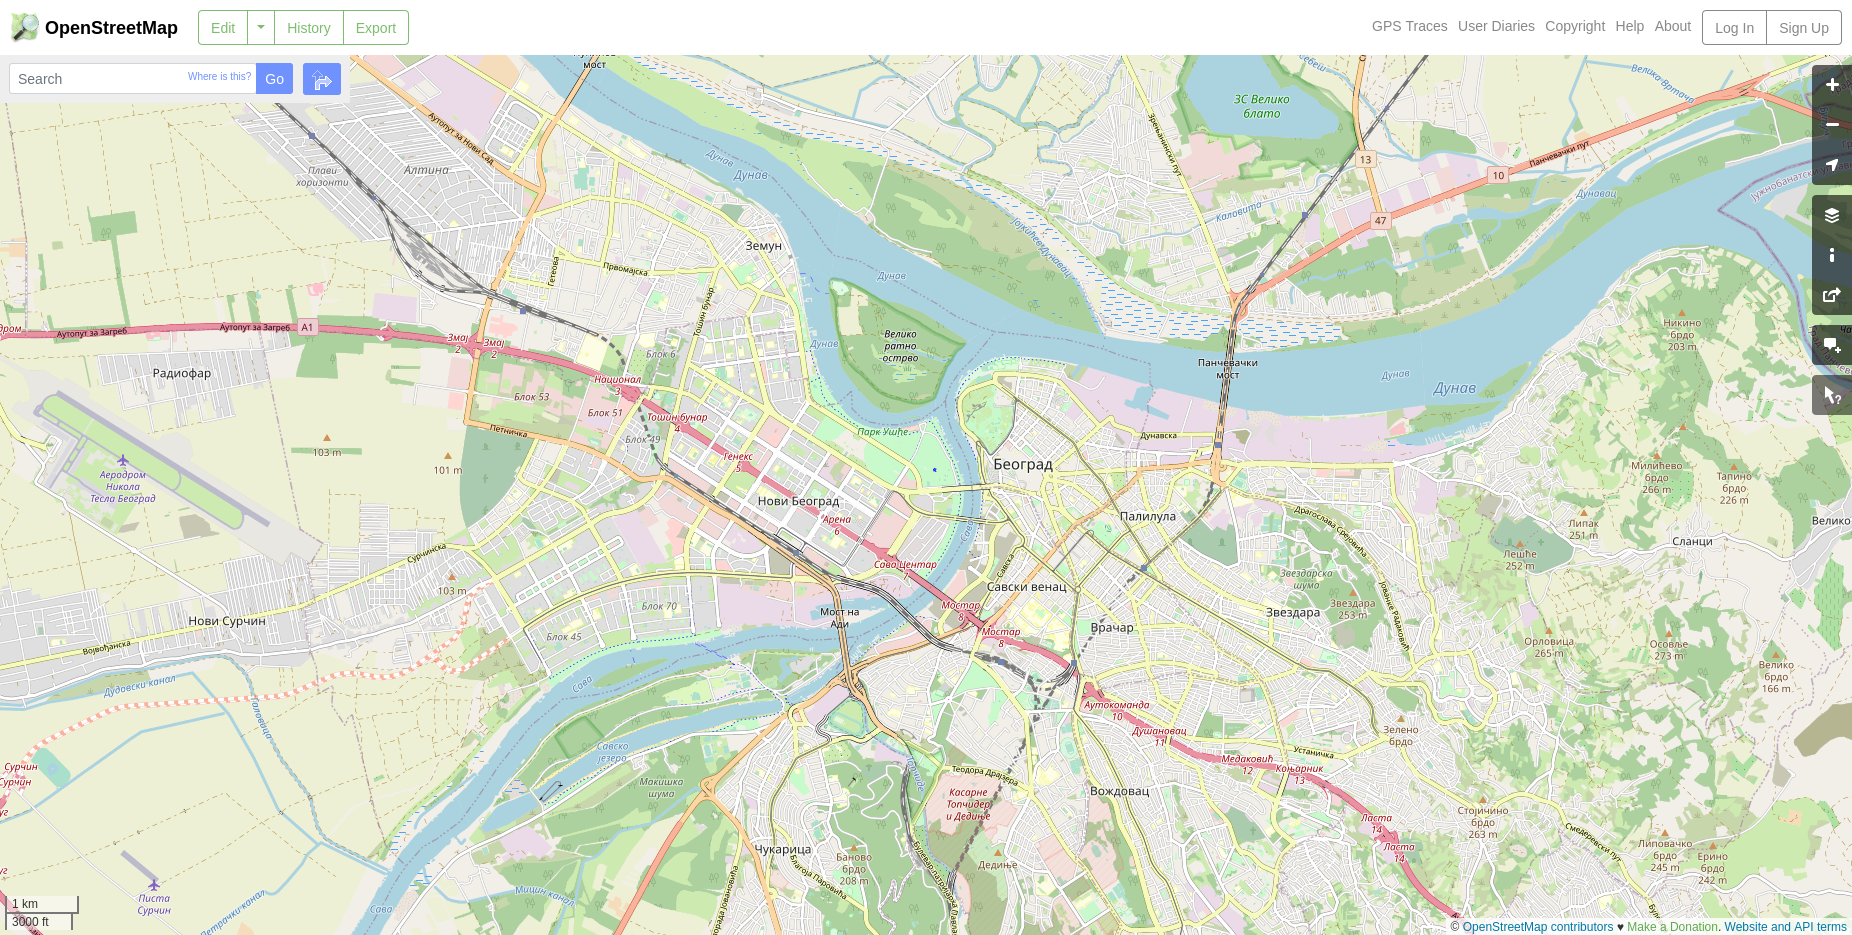
\includegraphics[width=1\textwidth]{pictures/osm_example.png}
  \caption{Приказ Београда у \textit{OSM}-у}
  \label{fig:osm_map_example}
\end{figure}

\textit{OSM} је 2004. године покренуо Стив Коуст (енг. \textit{Steve Coast}) са идејом креирања мапа за Уједињено Краљевство. У наредним годинама пројекат је постао глобалан и сада садржи податке целог света \cite{osm_wiki}.

\section{Елементи}
\label{sec:osm_elementi}

За моделовање података физичког света у оквиру \textit{OSM}-а се користе \textit{OSM} елементи \cite{osm_wiki}. Постоје три врсте елемената и то су чворови (енг. \textit{nodes}), путање (енг. \textit{ways}) и релације (енг. \textit{relations})

Сваки од елемената може имати придружен један или више тагова (енг. \textit{tag}) чија је улога да опишу елемент коме припадају. Елементи \textit{OSM} скупа се могу представити помоћу \textit{XML} записа од којих је сваки одређен засебним \textit{XML} тагом \cite{osm_xml}. Сваки елемент у \textit{XML} запису поседује атрибуте који га описују. Постоје одређени атрибути који се налазе у сваком елементу:

\begin{description}
	\item[\textit{id},] јединствен идентификатор елемента;
	\item[\textit{user},] име корисника који је изменио елемент;
	\item[\textit{uid},] идентификатор корисника који је изменио елемент;
	\item[\textit{timestamp},] време последње промене елемента;
	\item[\textit{visible},] знак који показује да ли је елемент видљив;
	\item[\textit{version},] тренутна верзија елемента (почетна вредност је 1 и сваки пут када се изврши модификација елемента тај број се инкрементира);
	\item[\textit{changeset},] идентификатор скупа промена у коме је елемент измењен.
\end{description}

\subsection{Тагови}
\label{subsec:osm_tags}

Тагови представљају опис \textit{OSM} елемента коме припадају. Сваки елемент може имати нула, један или више тагова \cite{osm_wiki}. Чине га две вредности, кључ, који мора бити јединствен унутар елемента ког таг описује, и вредност. У коду \ref{lst:osm_tag_xml} је приказан пример тагова у \textit{XML} формату. Кључ и вредност су означени редом атрибутима \textit{k} и \textit{v}. Приказани тагови припадају примеру чвора из кода \ref{lst:osm_node_xml} и показују да чвор представља саобраћајни знак.

\begin{lstlisting}[language=XML, caption={Пример \textit{OSM} тагова у \textit{XML} формату}, label={lst:osm_tag_xml}]
<tag k="name" v="Neu Broderstorf"/>
<tag k="traffic_sign" v="city_limit"/>
\end{lstlisting}

\section{Чворови}
\label{sec:osm_nodes}

Чвор представља локацију на Земљиној површини и састоји се од две координате које представљају географску дужину и ширину \cite{osm_wiki}. Један чвор се може користити за дефиницију објекта на мапи, попут, на пример, клупе, статуе или фонтане.

У језику \textit{XML} чворови су представљени \textit{XML} тагом \textit{node} унутар ког су угњеждени \textit{OSM} тагови који му припадају. К\^{о}д \ref{lst:osm_node_xml} представља један чвор записан у \textit{XML} формату. Атрибути \textit{lat} и \textit{lon} представљају координате чвора на мапи. Чвор садржи два тага, који означавају да се на координатама чвора налази саобраћајни знак који представља улазак у насеље \textit{Neu Broderstorf}.

\begin{lstlisting}[language=XML, caption={\textit{XML} запис \textit{OSM} чвора који представља саобраћајни знак}, label={lst:osm_node_xml}]
<node id="1831881213" version="1" changeset="12370172" lat="54.0900666" lon="12.2539381" user="lafkor" uid="75625" visible="true" timestamp="2012-07-20T09:43:19Z">
  <tag k="name" v="Neu Broderstorf"/>
  <tag k="traffic_sign" v="city_limit"/>
 </node>
\end{lstlisting}

\section{Путање}
\label{sec:osm_ways}

Путање су уређене листе које садрже између 2 и 20000 чворова и представљају линеарне објекте на мапи, попут путева или река \cite{osm_wiki}. Такође, могу представљати и разне врсте површина, попут шума. У том случају су први и последњи елемент листе исти чвор. 

Путање су у \textit{XML} формату представљене листом идентификатора чворова које та путања садржи. Сваки чвор путање је записан \textit{XML} тагом \textit{nd} са атрибутом \textit{ref} унутар ког се налази идентификатор чвора. Поред идентификатора чворова, путања може садржати и \textit{OSM} тагове. \textit{XML} таг који означава путању је \textit{way}. У коду \ref{lst:osm_way_xml} је приказан пример путање која представља ауто-пут. Унутар \textit{OSM} тагова путање је записано име улице, као и информација о томе да је ауто-пут једносмеран.

\begin{lstlisting}[language=XML, caption={\textit{XML} запис \textit{OSM} путањe која представља ауто-пут}, label={lst:osm_way_xml}]
<way id="5090250" visible="true" timestamp="2009-01-19T19:07:25Z" version="8" changeset="816806" user="Blumpsy" uid="64226">
    <nd ref="822403"/>
    <nd ref="21533912"/>
    <nd ref="821601"/>
    <nd ref="21533910"/>
    <nd ref="135791608"/>
    <nd ref="333725784"/>
    <nd ref="333725781"/>
    <nd ref="333725774"/>
    <nd ref="333725776"/>
    <nd ref="823771"/>
    <tag k="highway" v="residential"/>
    <tag k="name" v="Clipstone Street"/>
    <tag k="oneway" v="yes"/>
  </way>
\end{lstlisting}

\section{Релације}
\label{sec:osm_relations}

Релације су структуре које представљају однос између \textit{OSM} елемената \cite{osm_wiki}. Могу имати разна значења па су због тога описане таговима. Обично, свака релација поседује \textit{OSM} таг који се зове \textit{type} и сваки други таг те релације се интерпретира на основу његове вредности.

У \textit{XML} формату, релација се означава тагом \textit{relation} и садржи чланове релације и \textit{OSM} тагове. Члан је одређен \textit{XML} тагом \textit{member} и садржи три атрибута:

\begin{description}
	\item[\textit{type},] \textit{OSM} тип члана, може бити \textit{node}, \textit{way} или \textit{relation};
	\item[\textit{ref},] идентификатор елемента члана;
	\item[\textit{role},] улога члана у релацији.
\end{description}

\textit{XML} репрезентација релације која представља аутобуску линију приказана је у коду \ref{lst:osm_relation_xml}. У овом примеру, \textit{OSM} чворови који припадају релацији представљају аутобуске станице. Поред чворова, релацији припада и једна путања, која приказује путању аутобуске линије. Тагови релације приказују почетну и завршну локацију линије, као и информације о превознику.

\begin{lstlisting}[language=XML, caption={\textit{XML} запис \textit{OSM} релације која представља аутобуску линију}, label={lst:osm_relation_xml}]
<relation id="13092746" visible="true" version="7" changeset="118825758" timestamp="2022-03-23T15:05:48Z" user="" uid="">
  <member type="node" ref="5690770815" role="stop"/>
  <member type="node" ref="5751940550" role="stop"/>
  ...
  <member type="node" ref="1764649495" role="stop"/>
  <member type="way" ref="96562914" role=""/>
  ...
  <member type="way" ref="928474550" role=""/>
  <tag k="from" v="Encre"/>
  <tag k="name" v="9-Montagnes de Guyane"/>
  <tag k="network" v="Agglo'bus"/>
  <tag k="not:network:wikidata" v="Q3537943"/>
  <tag k="operator" v="CACL"/>
  <tag k="ref" v="9"/>
  <tag k="route" v="bus"/>
  <tag k="to" v="Lyce Balata"/>
  <tag k="type" v="route"/>
 </relation>
\end{lstlisting}

% ============== ??? =====================
% pomeni leaflet za prikaz mapa. Ali to moze da se uradi u aplikacija sekciji
% mozda pasus za semanticki veb + osm. Ali to mozda i u zakljucku: https://wiki.openstreetmap.org/wiki/OSM_Semantic_Network
% ============== ??? =====================

\chapter{App}
\label{chp:app}

\section{Opis}
\label{sec:opis}

ovde opis appa i sta se trazi od nas

\section{Cloud}
\label{sec:cloud}

шта је cloud и које услуге нуди. EMR, EC2, S3 нпр мало детаљније. За ово или ова секција или одвојена, након дистрибуираних система.

\section{Arhitektura aplikacije}
\label{sec:app_aphi}

opis komponenti

\section{Подаци}
\label{sec:osm_spark_podaci}

skupovi podataka koji se koriste mada je vecina toga vec napisana ranije, u OSM delu. Dakle OSM + geonames

\section{Obrada OSM skupa Sparkom}
\label{sec:osm_spark_obrada}

koje spark transformacije su primenjene na koje podatke

\section{PolyContains}
\label{sec:poly_cont}

algoritmi korisceni za poly contains i rezultati (graficki prikaz). mozda zameniti mesta ovoj i prethodnoj sekciji...

\section{Rezultat}
\label{sec:rezultat}

dobijeni rezultati aplikacije, prikaz nekih selekcija itd

\chapter{Закључак}
\label{chp:zakljucak}

zakljucak rada. Takodje, uvod treba da se uradi

% potencijalne nadogradnje:
% napraviti da radi za posebne gradove/regije/pokrajne
% nadograditi da radi sa semantickim vebom mozda

% ------------------------------------------------------------------------------
% Literatura
% ------------------------------------------------------------------------------
\literatura

% ==============================================================================
% Završni deo teze i prilozi
\backmatter
% ==============================================================================

% ------------------------------------------------------------------------------
% Biografija kandidata
\begin{biografija}
\textbf{Вук Стефановић Караџић} (\emph{Тршић, 26. октобар/6. новембар
  1787. — Беч, 7. фебруар 1864.}) био је српски филолог, реформатор
српског језика, сакупљач народних умотворина и писац првог речника
српског језика.  Вук је најзначајнија личност српске књижевности прве
половине XIX века. Стекао је и неколико почасних доктората.
Учествовао је у Првом српском устанку као писар и чиновник у
Неготинској крајини, а након слома устанка преселио се у Беч,
1813. године. Ту је упознао Јернеја Копитара, цензора словенских
књига, на чији је подстицај кренуо у прикупљање српских народних
песама, реформу ћирилице и борбу за увођење народног језика у српску
књижевност. Вуковим реформама у српски језик је уведен фонетски
правопис, а српски језик је потиснуо славеносрпски језик који је у то
време био језик образованих људи. Тако се као најважније године Вукове
реформе истичу 1818., 1836., 1839., 1847. и 1852.
\end{biografija}
% ------------------------------------------------------------------------------

\end{document} 